
\section{Unfolding jet response}
\label{sec:jetunfolding}
\subsection{Truth-Reco matching}
Jet matching adapted from CMS ``algorithmic definition" is used extensively in HEP/pp analyses that use flavor tagging. For example, see \url{https://twiki.cern.ch/twiki/bin/view/CMSPublic/BtagRecommendation2010OpenData}. In this method, reconstructed jets are filled with generator truth particles, tagged via fastjet::PseudoJet::set\_user\_index(n), $n \geq 0$, according to their ownership by generator truth jet $n$. The association is made through the highest {$z_{T}^{\mathrm{tag}}\equiv\sum p_{T}^{\mathrm{tag}}/ \sum p_{T}^{\mathrm{reco}}$}. 

The truth particles are clustered into the anti-$k_T$ jets as ghosts,
where the energy--momentum is scaled by the factor $2^{-30}$ (a factor
that numerically, once multiplied, is recoverable without incurring
rounding effects). The matching preference between the truth jet
$J_{\mathrm{truth},k}$ and reco jet $J_{\mathrm{reco},l}$ is given by
\begin{equation}
  z_{\mathrm{reco},kl} = \frac{\sum_{j \in J_{\mathrm{truth},k} \cup
      J_{\mathrm{reco},l}} p_{T,j}}{\sum_{j \in J_{\mathrm{reco},l}}
    p_{T,j}}
\end{equation}
which is the fraction of truth constituents of a particular MC truth
jet inside the catchment area of the reco jet, relative to the sum of
total MC truth particles inside the catchment area of the reco jet.

Figure~\ref{fig:zmatching_reco} shows the resulting $z_{\mathrm{reco}}$ for the matched jets (i.e. highest $z_{\mathrm{reco}}$) for photon+jet simulations in pp and p-Pb data. The jets shown have reconstructed pseudorapidity $|\eta^{\mathrm{jet}}_{\mathrm{reco}}|<0.5$ and transverse momentum $p_{\mathrm{T}}^{\mathrm{sub}}> 10$ \GeVc, and are recoiling ($\Delta\varphi > \pi/2$) against an isolated photon with momentum 20--30 \GeVc~that passes our event selection. 

\begin{figure}
\center
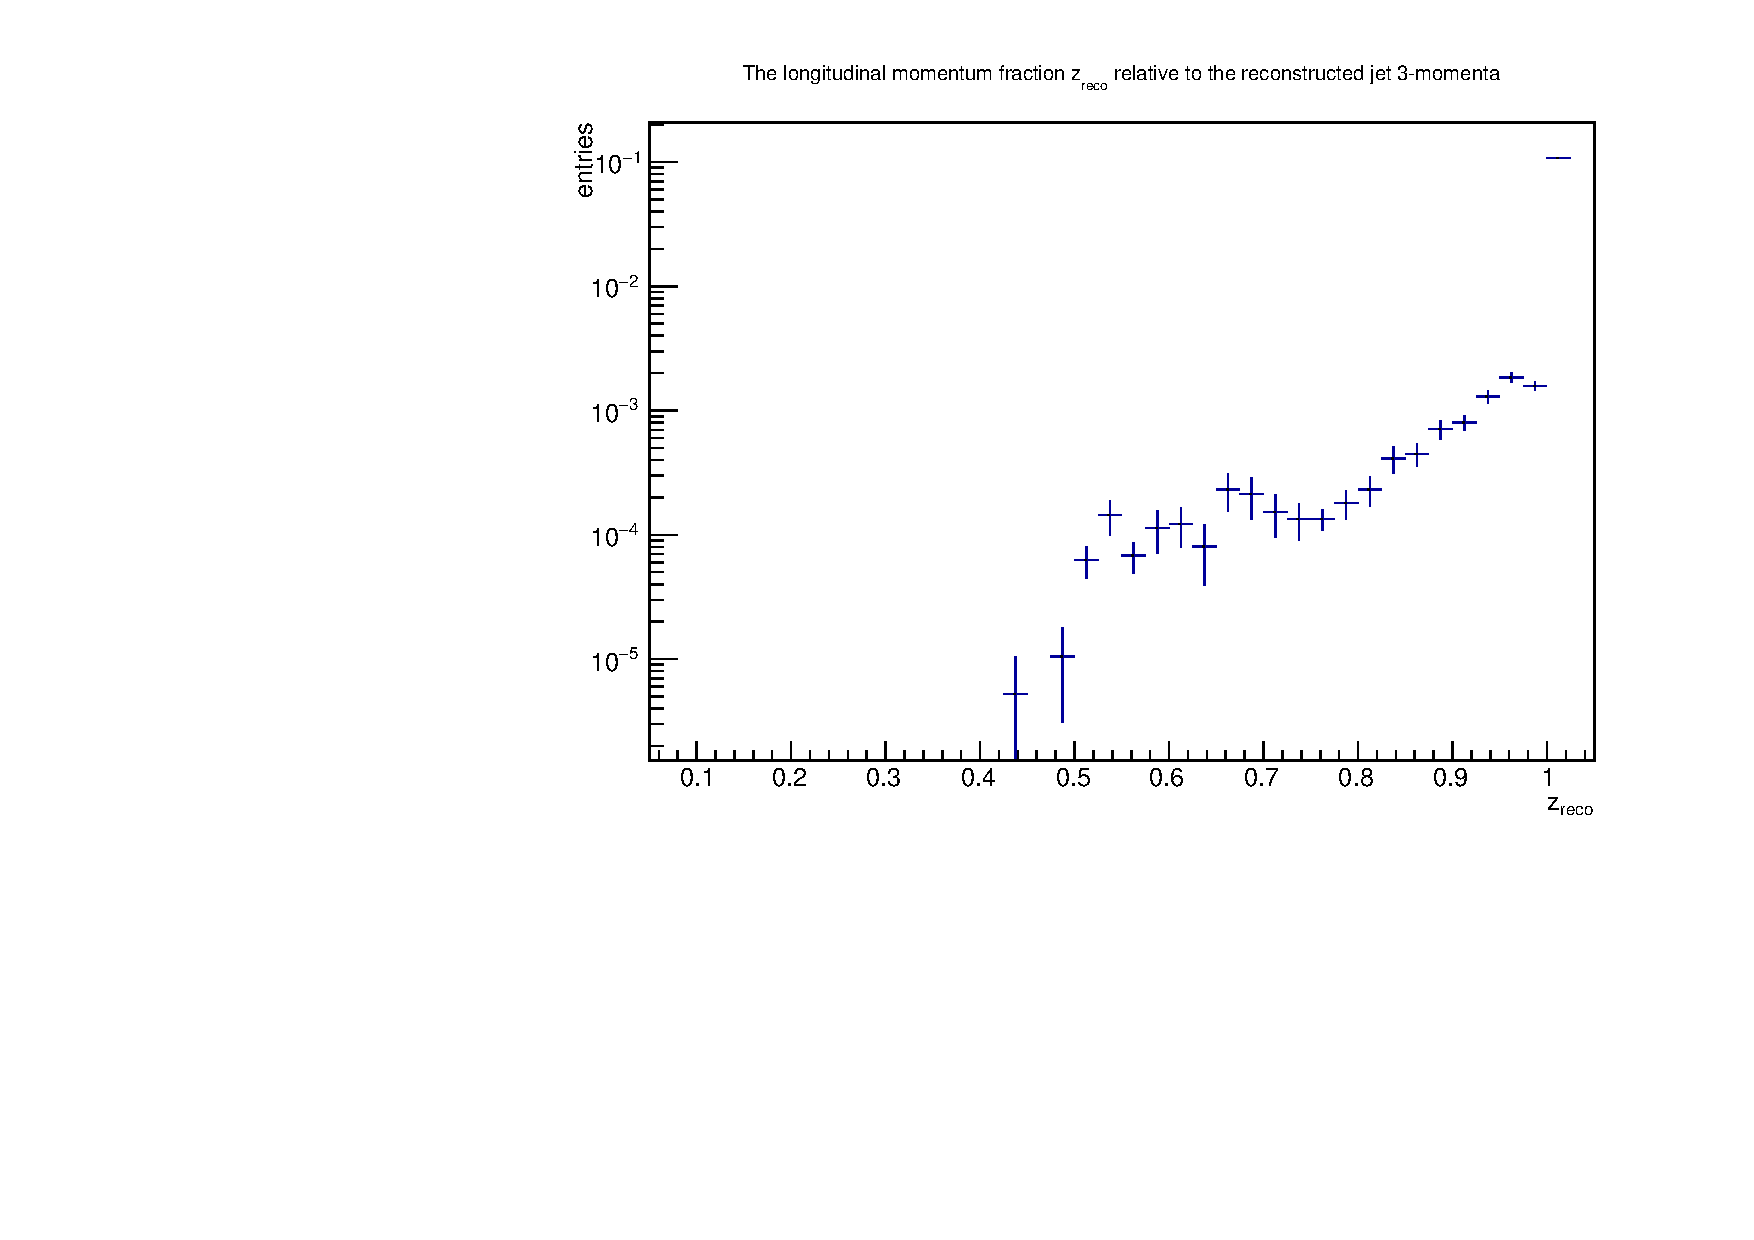
\includegraphics[width=0.49\textwidth]{JetReco/zreco_pPb}
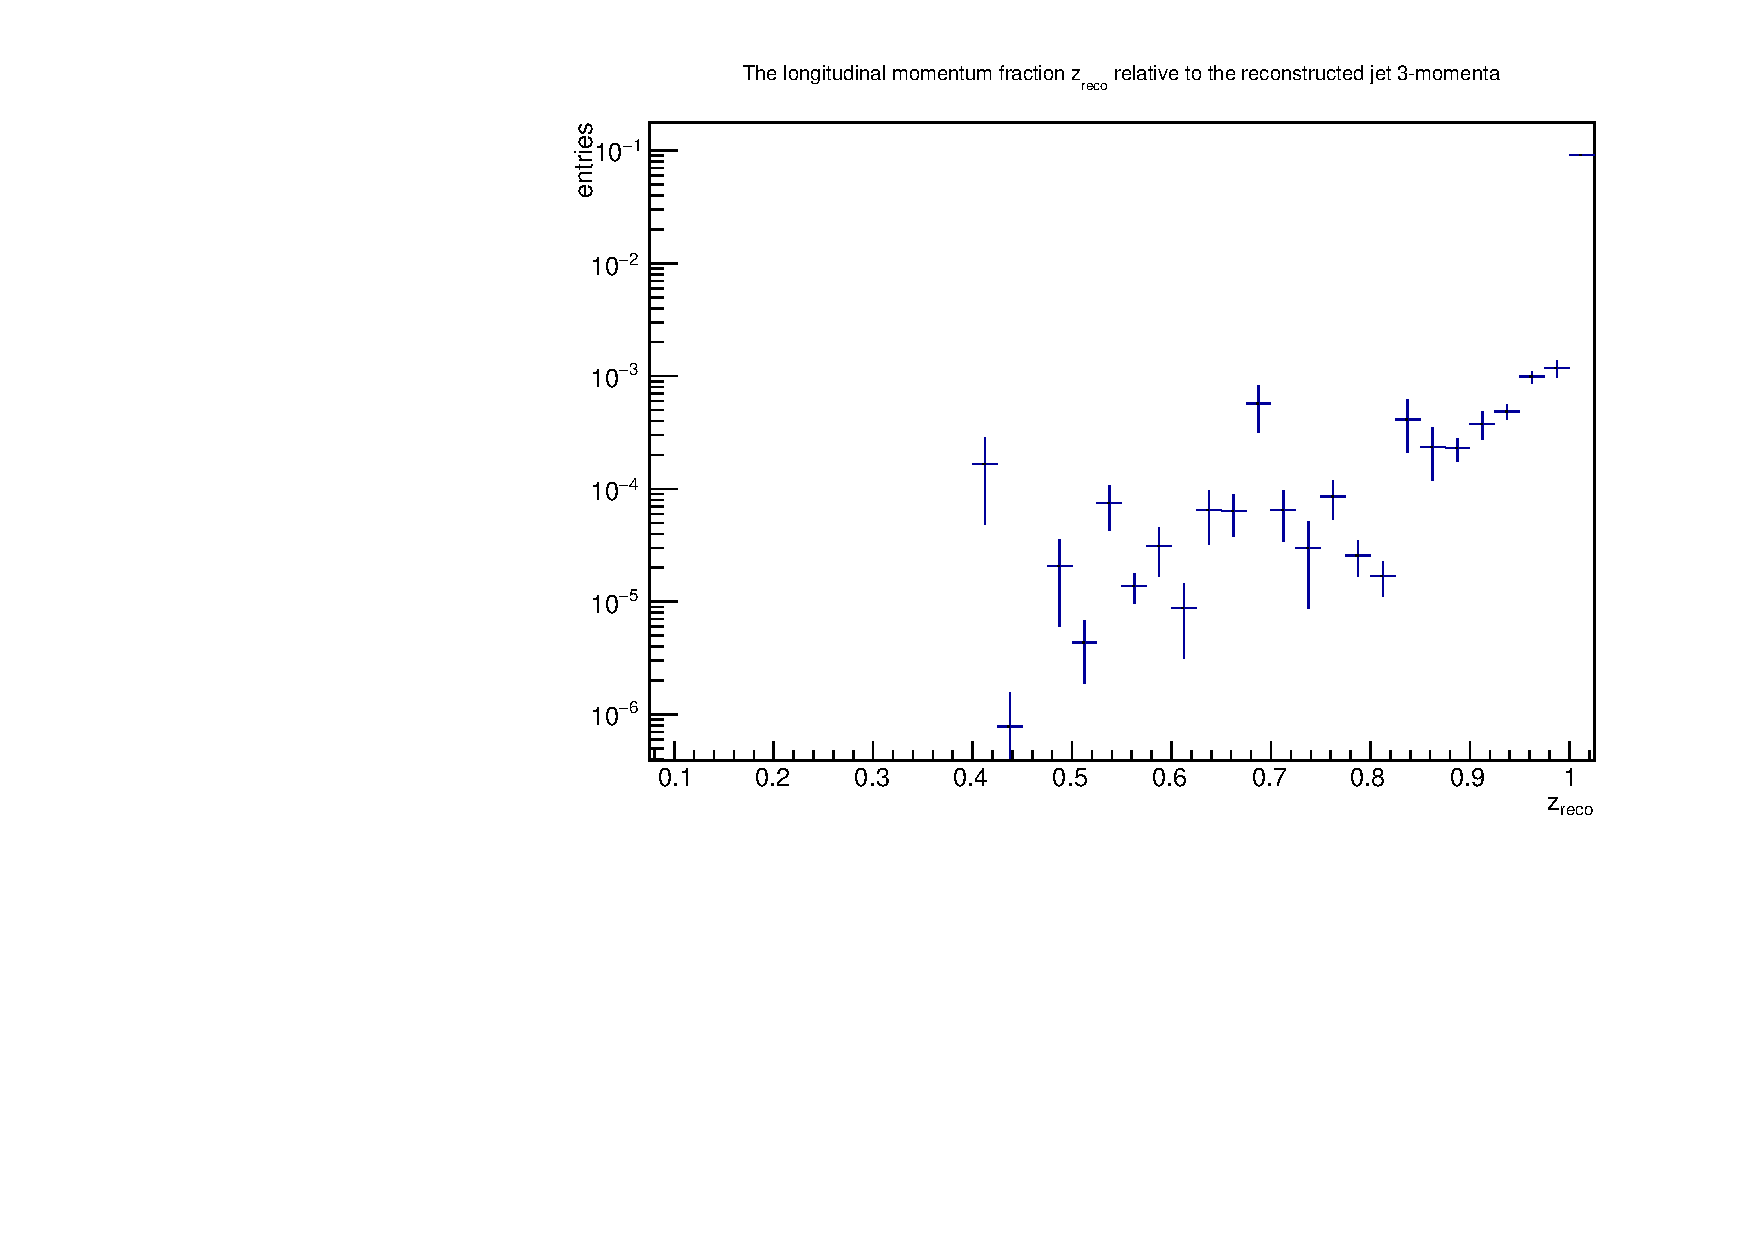
\includegraphics[width=0.49\textwidth]{JetReco/zreco_pp}\\
\label{fig:zmatching_reco}
\caption{The longitudinal momentum fraction $z_{\mathrm{reco}}$ for matched jets, relative to the reconstructed jet 3-momenta. The left panel represents photon+jet simulation in p-Pb data the right panel shows the results for photon+jet simulation for pp data. The jets shown here have $|\eta^{\mathrm{jet}}_{\mathrm{reco}}|<0.5$ and $p_{\mathrm{T}}^{\mathrm{sub}}> 10$ \GeVc.}
\end{figure}

Note that by nature of the detector inefficiencies and edges, this
(inverse appearing, reco-to-truth) definition is not symmetric. If the
denominator would be replaced by $J_{\mathrm{truth},l}$, i.e:

\begin{equation}
  z_{\mathrm{truth},kl} = \frac{\sum_{j \in J_{\mathrm{truth},k} \cup
      J_{\mathrm{reco},l}} p_{T,j}}{\sum_{j \in J_{\mathrm{truth},l}}
    p_{T,j}}, 
\end{equation}
small area jets will be favored, which can easily deposit all particles inside
the catchment area of the reco jets, while the kinematics of observed
reco jet is not representative of this small truth jet.

Figure~\ref{fig:ztruthmatching} shows the  shows the corresponding resulting $z_{\mathrm{truth}}$ distribution. 

\begin{figure}
\center
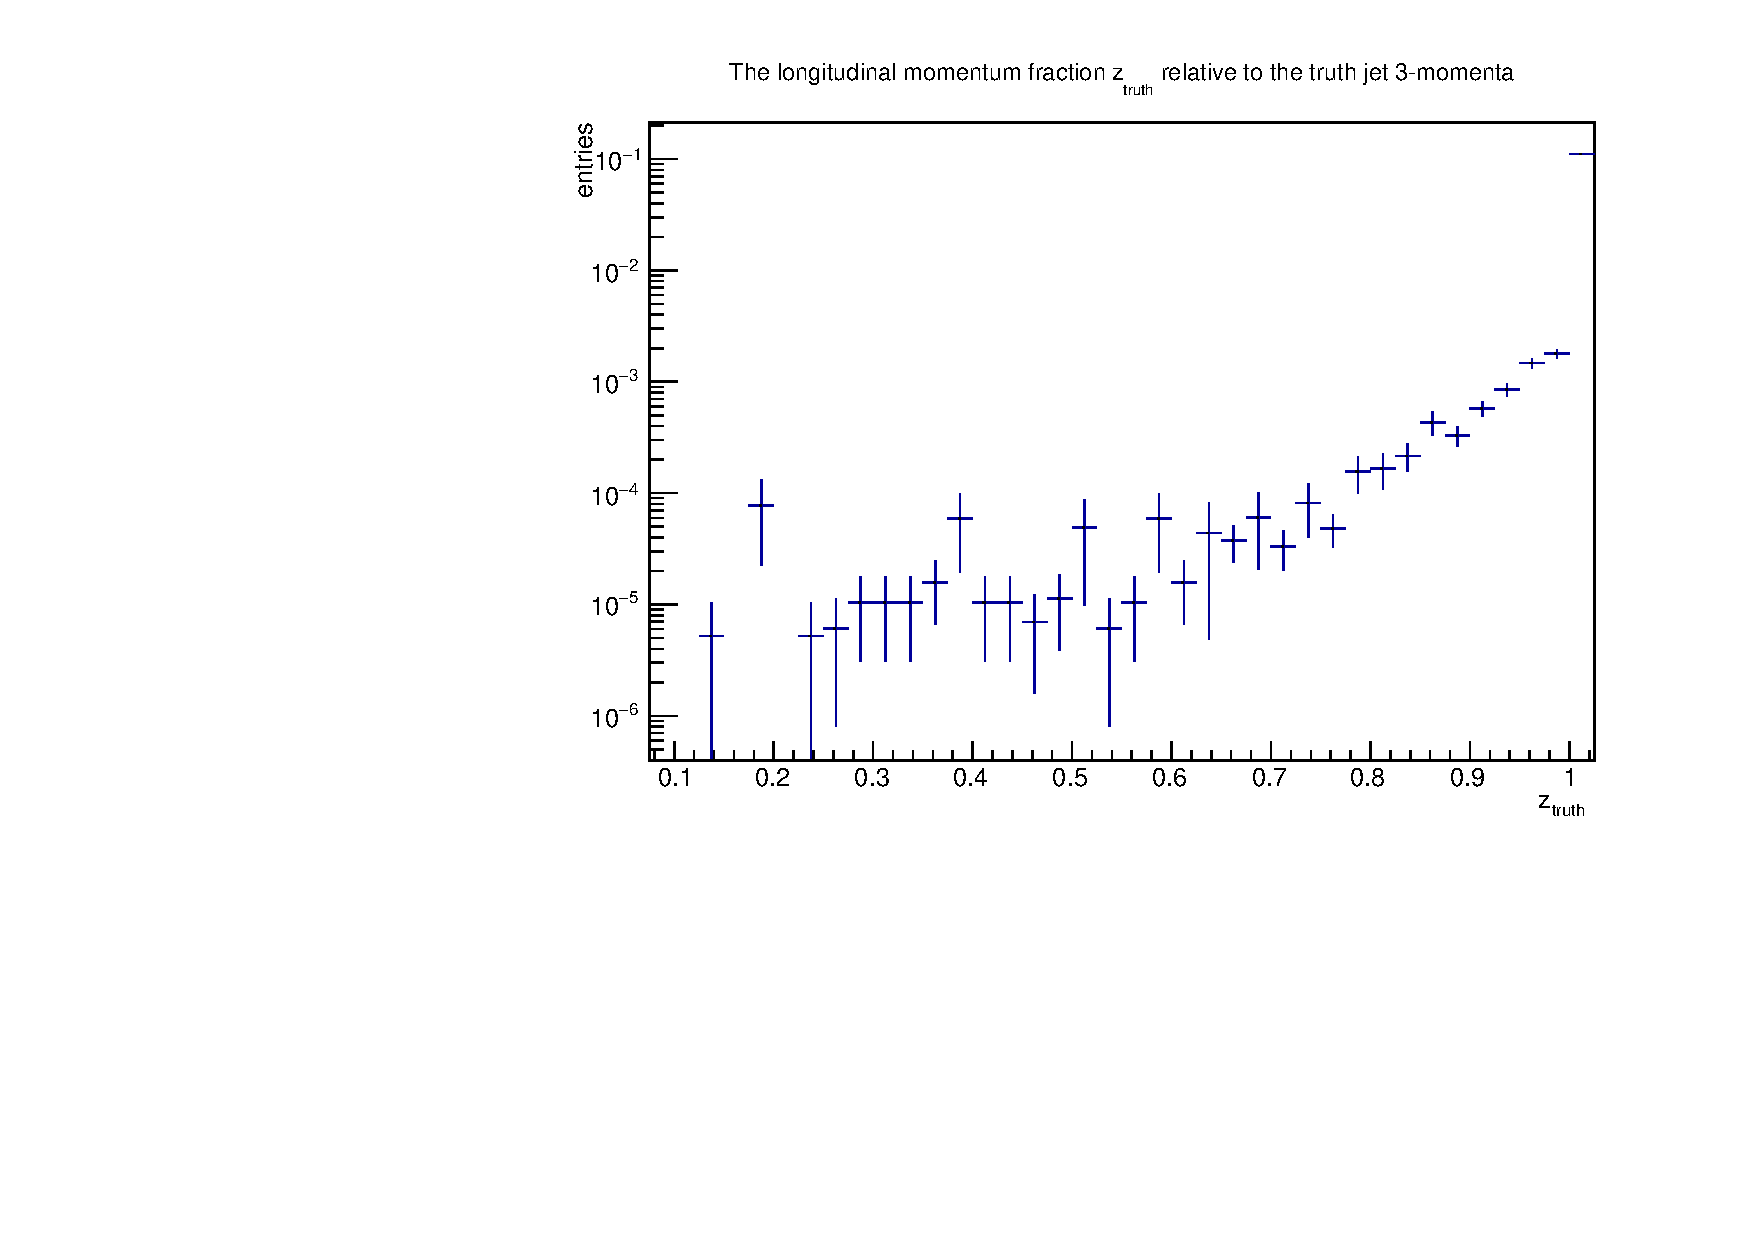
\includegraphics[width=0.49\textwidth]{JetReco/ztruth_pPb}
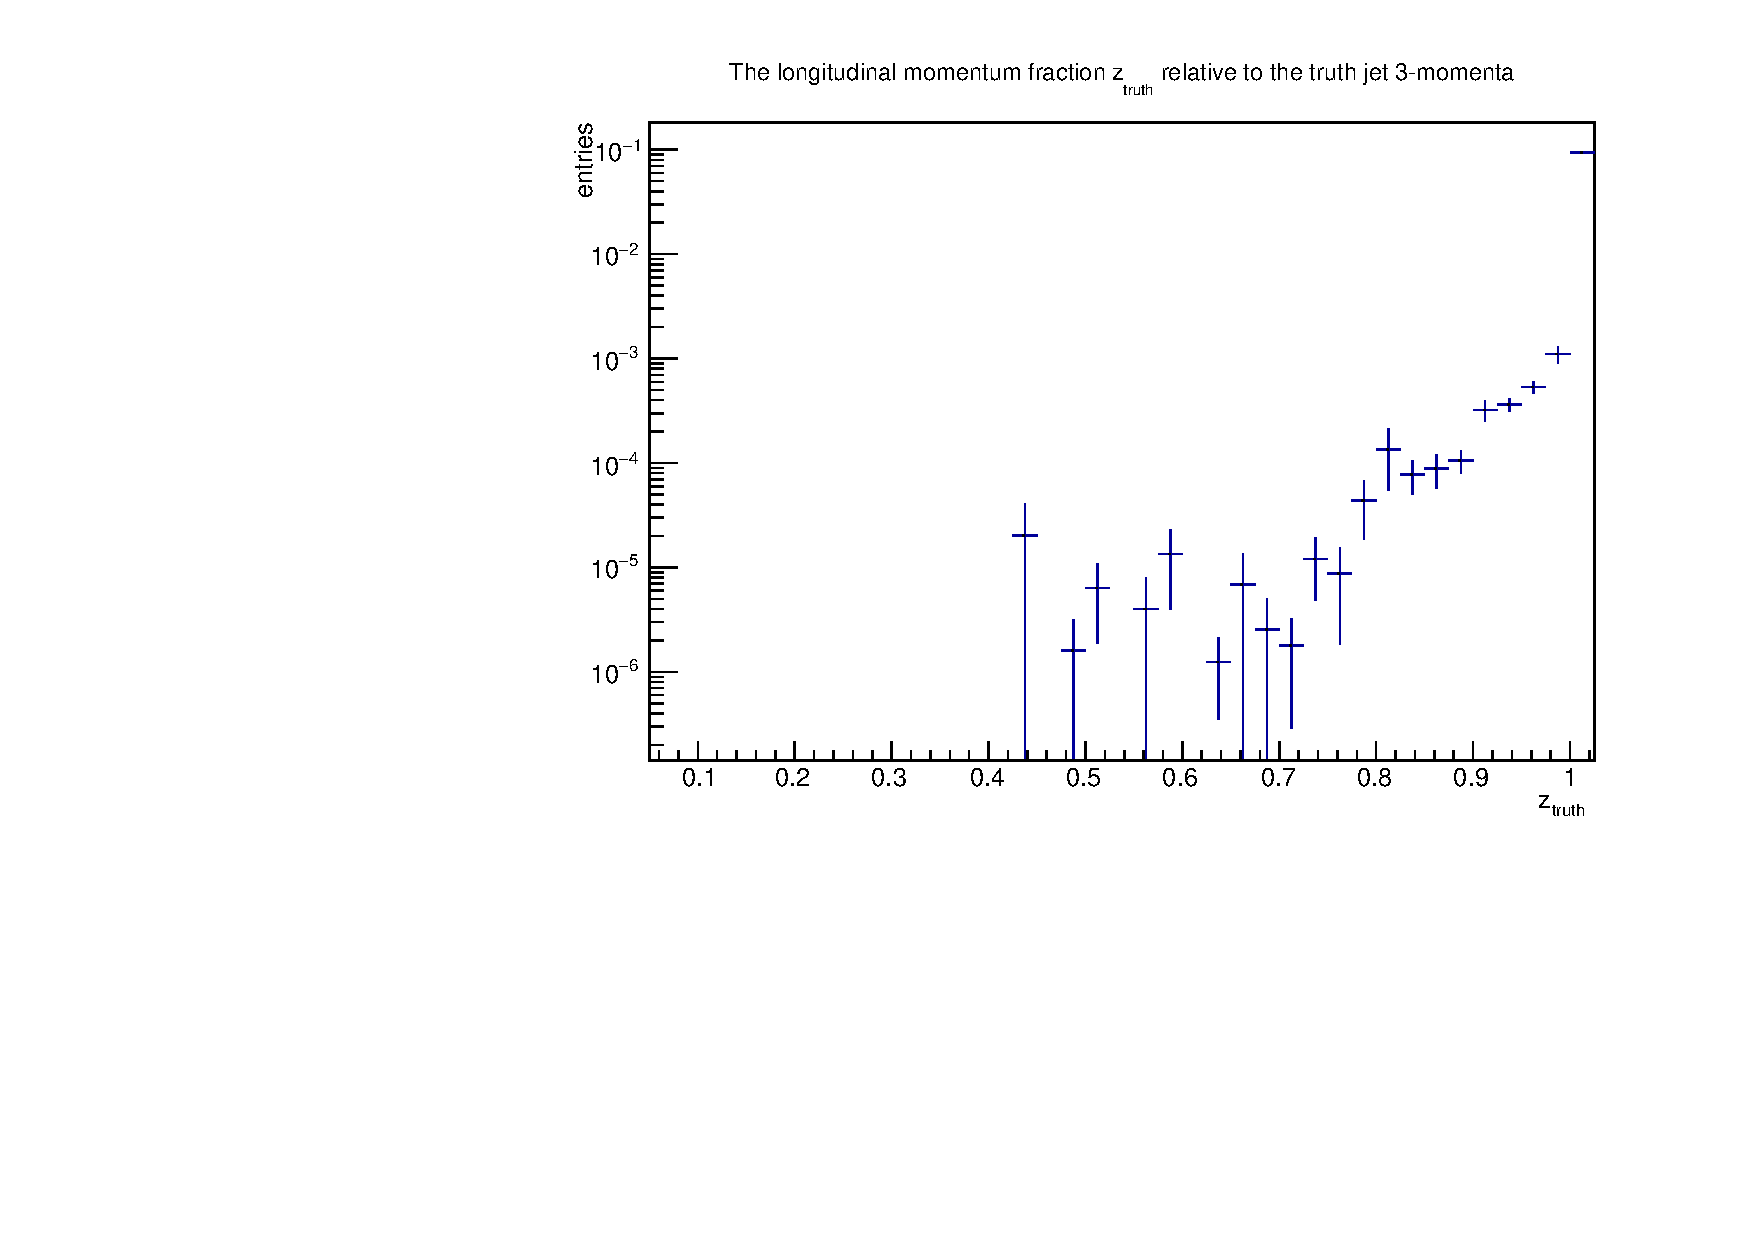
\includegraphics[width=0.49\textwidth]{JetReco/ztruth_pp}\\
\label{fig:ztruthmatching}
\caption{The longitudinal momentum fraction $z_{\mathrm{truth}}$ for matched jets, relative to the truth jet 3-momenta. The left panel represents photon+jet simulation in p-Pb data the right panel shows the results for photon+jet simulation for pp data. The jets shown here have $|\eta^{\mathrm{jet}}_{\mathrm{reco}}|<0.5$ and $p_{\mathrm{T}}^{\mathrm{sub}}> 10$ \GeVc.}
\end{figure}

In all cases the fraction of reconstructed jets that have at least 50$\%$ of the true jet momentum (in terms of true constituents) is larger than 99$\%$. 

\FloatBarrier
\subsection{Unfolding procedure}
\label{sec:unfolding}
The corrected signal yield is unfolded using the iterative D\textquotesingle Agostini method~\cite{DAgostini:1994fjx}, as implemented in the \textsc{RooUnfold} software package~\cite{Adye:2011gm}, to take into account migrations between different bins due to the jet energy scale and resolution. The unfolding response matrix from the~\textsc{Pythia} photon+jet sample, for jets reconstructed with ITS-only tracking is shown in Figure~\ref{fig:JetPTUnfolding}.
\begin{figure}
\center
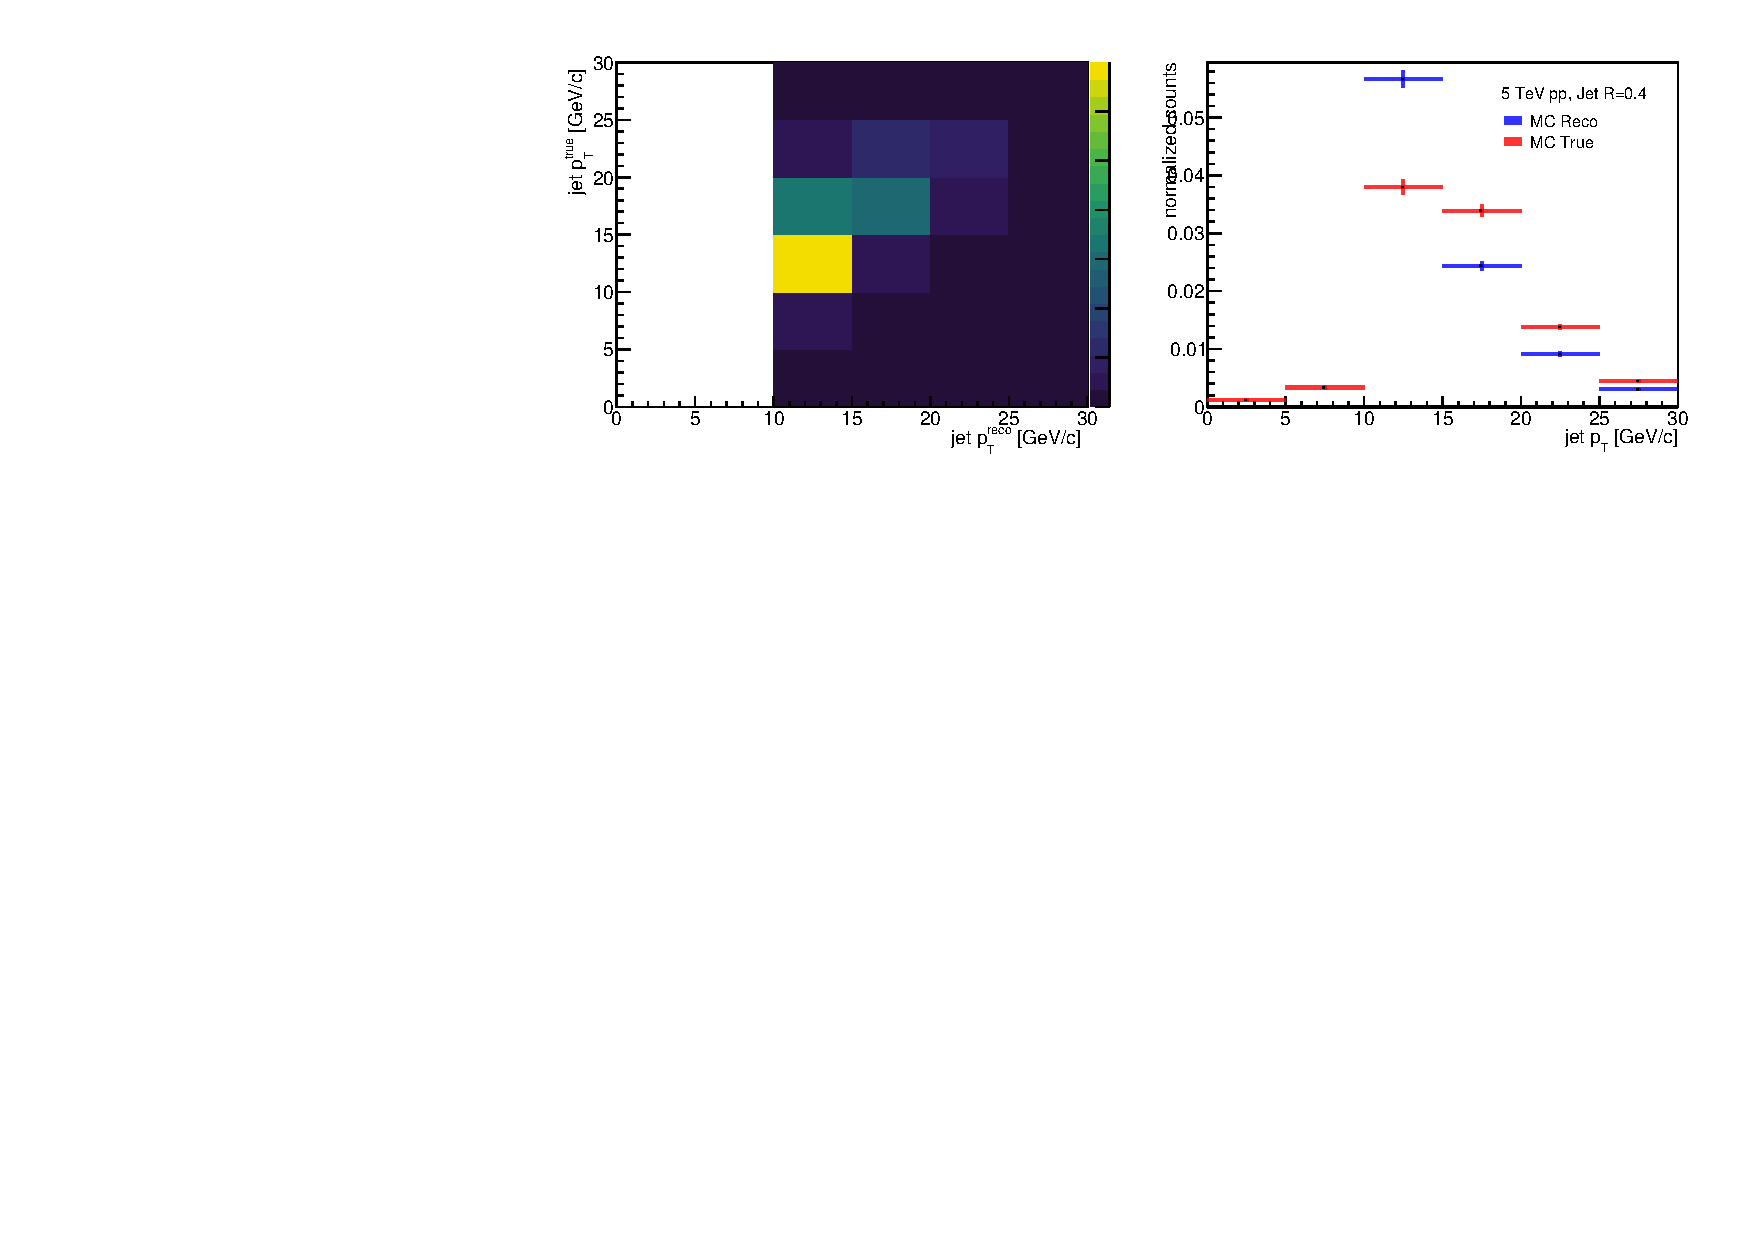
\includegraphics[width=0.99\textwidth]{JetResponse/UnfoldingMatrixpp}\\
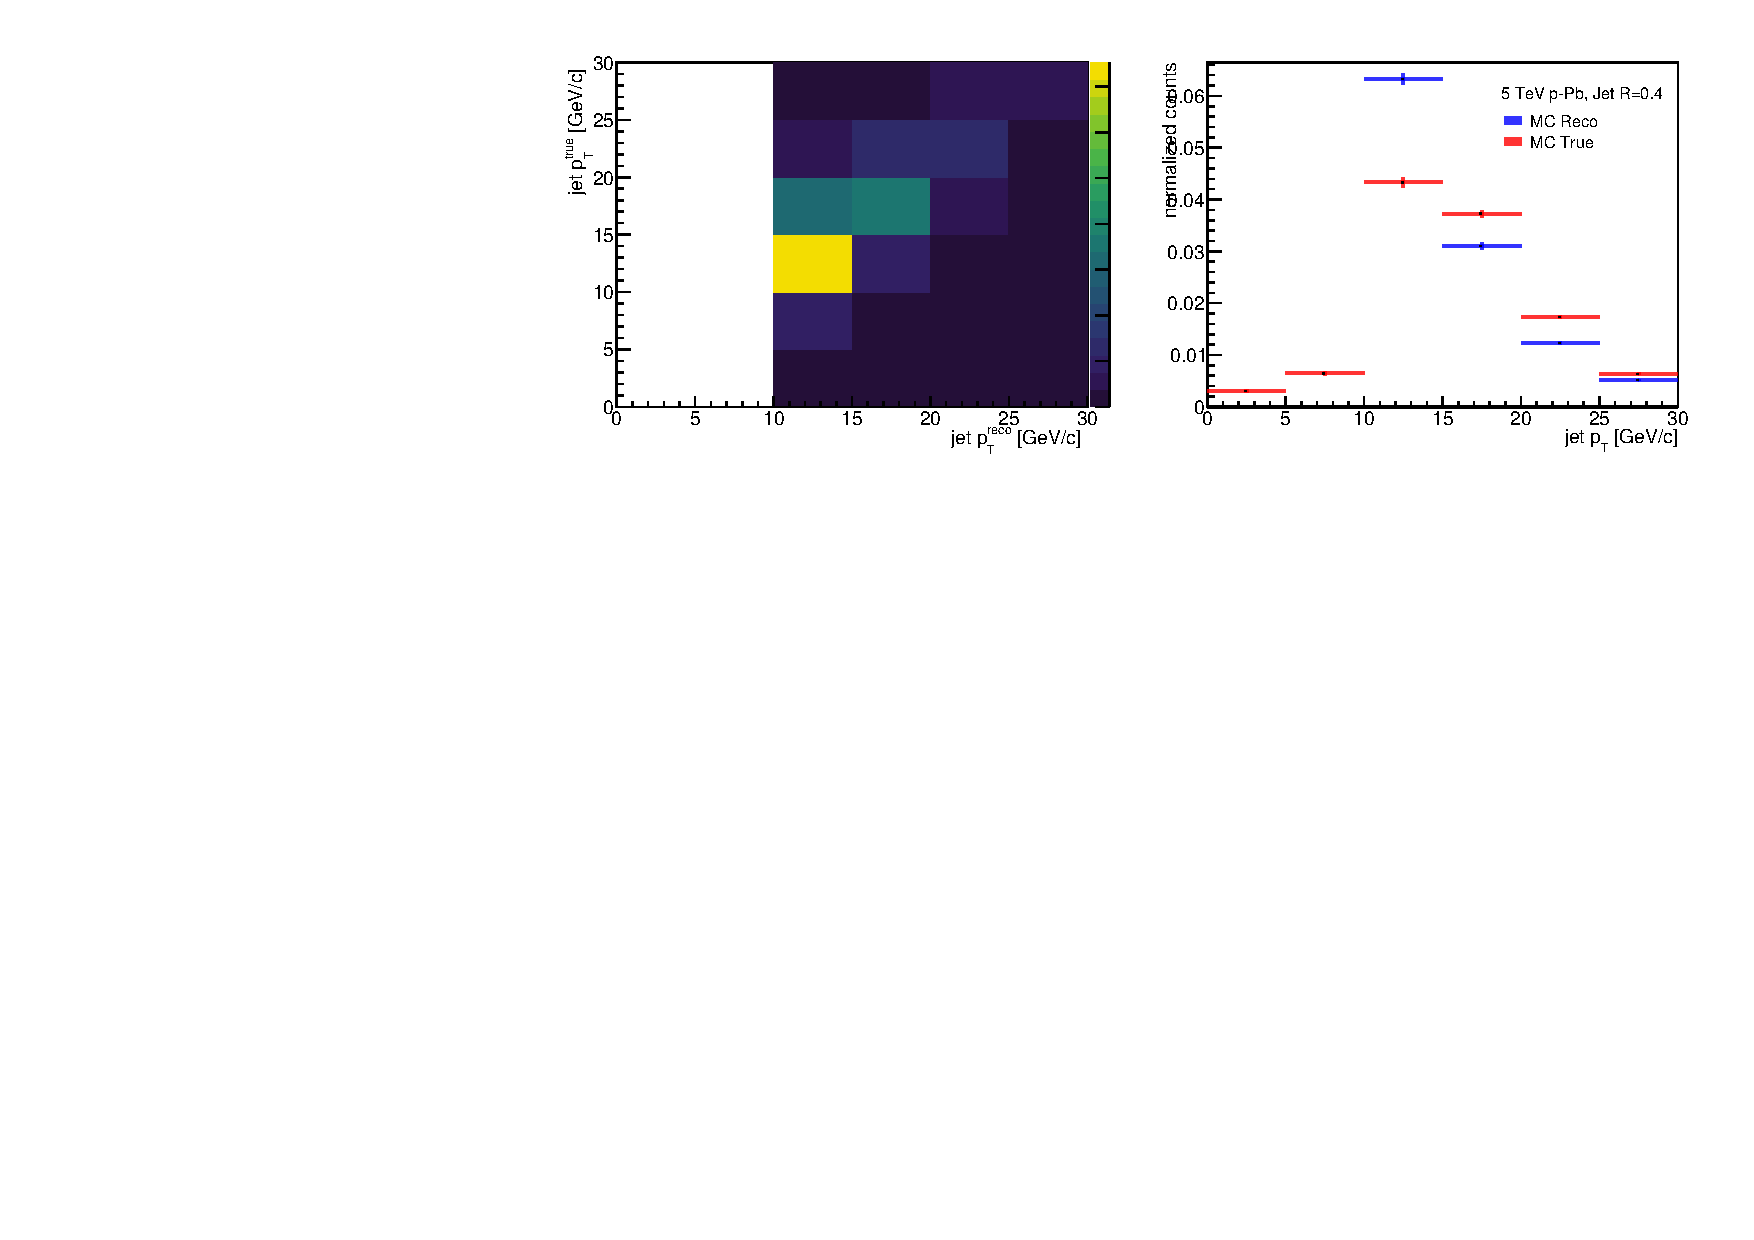
\includegraphics[width=0.99\textwidth]{JetResponse/UnfoldingMatrixpPb}\\
\caption{Left panel: Response matrix for jet $\pt$ measurement from photon+jet simulation. Right panel: Projection of response matrix. The first row corresponds to pp photon+jet simulation and the bottom row to p-Pb photon+jet simulation. The jets have $|\eta^{\mathrm{reco}}|<0.5$. The error bars represent statistical uncertainty only.}
\label{fig:JetPTUnfolding}
\end{figure}

As shown in Section~\ref{sec:jetresponse}, the ITS-only single-track resolution results in significant smearing effects for jets reconstructed with ITS-only tracks. Here, we apply a lower cut off {10 \GeVc~} for reconstructed jet $\pt$, which is the threshold we apply in the analysis. The projections of the response matrix show the impact of momentum smearing. The hard cut of 10 \GeVc~at the reconstructed level translates to the generated level as a distribution that peaks around 10~\GeVc~but has a a non-negligible left tail.

For illustration purposes, the response matrix is truncated for the region $\pt^{\mathrm{true}}<30$ GeV and $\pt^{\mathrm{reco}}<30$ GeV, but the overflow regions are actually used in the unfolding procedure by using the \textsc{RooUnfoldResponse::UseOverflow()}. The statistical uncertainty of the response matrix is taken into account by using the \textsc{RooUnfold::IncludeSystematics()} method.

Figure~\ref{fig:kinematic_efficiency} shows the ``kinematic efficiency'', defined as the ratio of truth jets matched to reconstructed jets with $\pt^{\mathrm{reco}}>10$ \GeVc~and $|\eta^{\mathrm{reco}}|<0.5$ to the total number of generated jets with $|\eta^{\mathrm{true}}|<0.5$. The kinematic efficiency has a rise to slightly above 10 \GeVc, as expected, and it reaches a plateau value of about 80$\%$. The left tail, which shows non-negligible efficiency to reconstruct jets with lower $\pt^{\mathrm{true}}$ than the threshold of $\pt>10$ \GeVc~at reconstructed level, arises due to bin migrations. 
\begin{figure}
\center
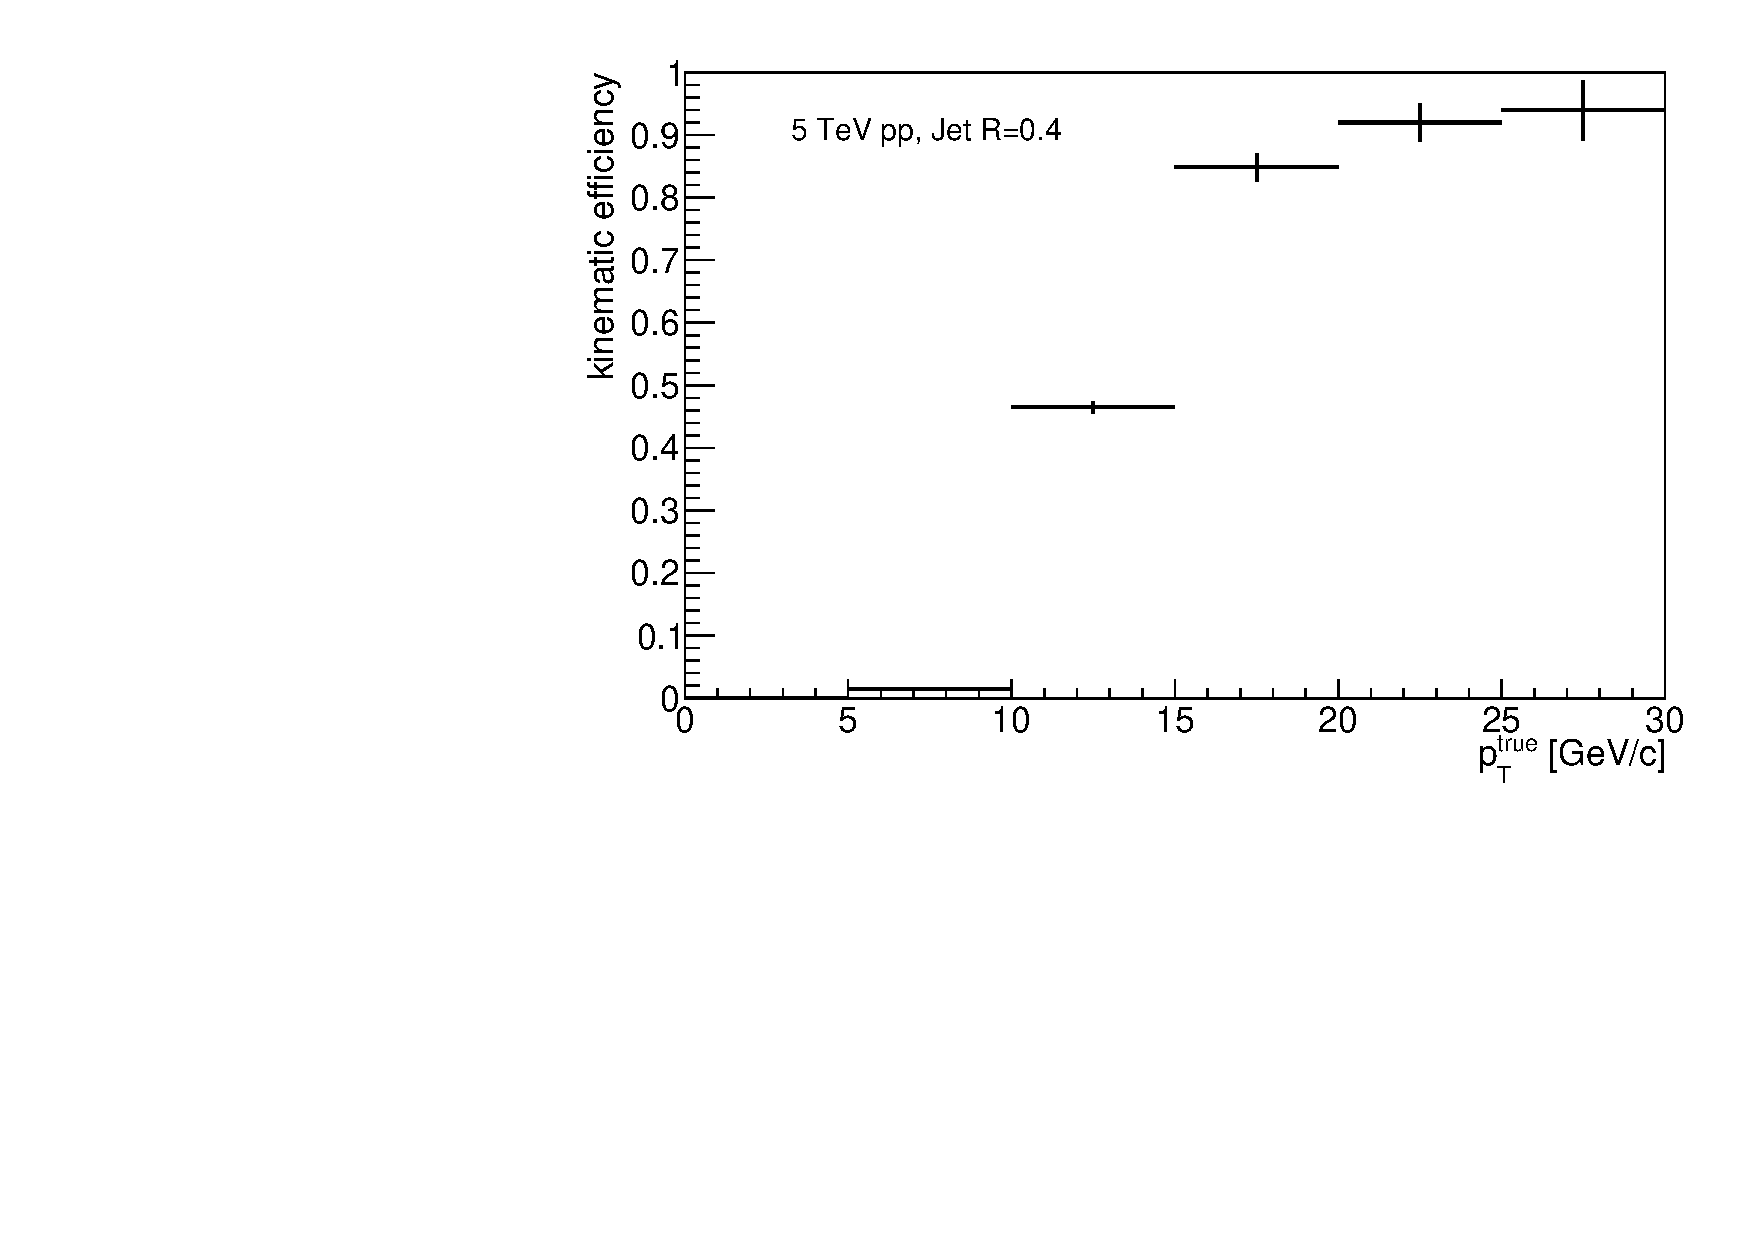
\includegraphics[width=0.49\textwidth]{JetResponse/KinematicEfficiencypp}
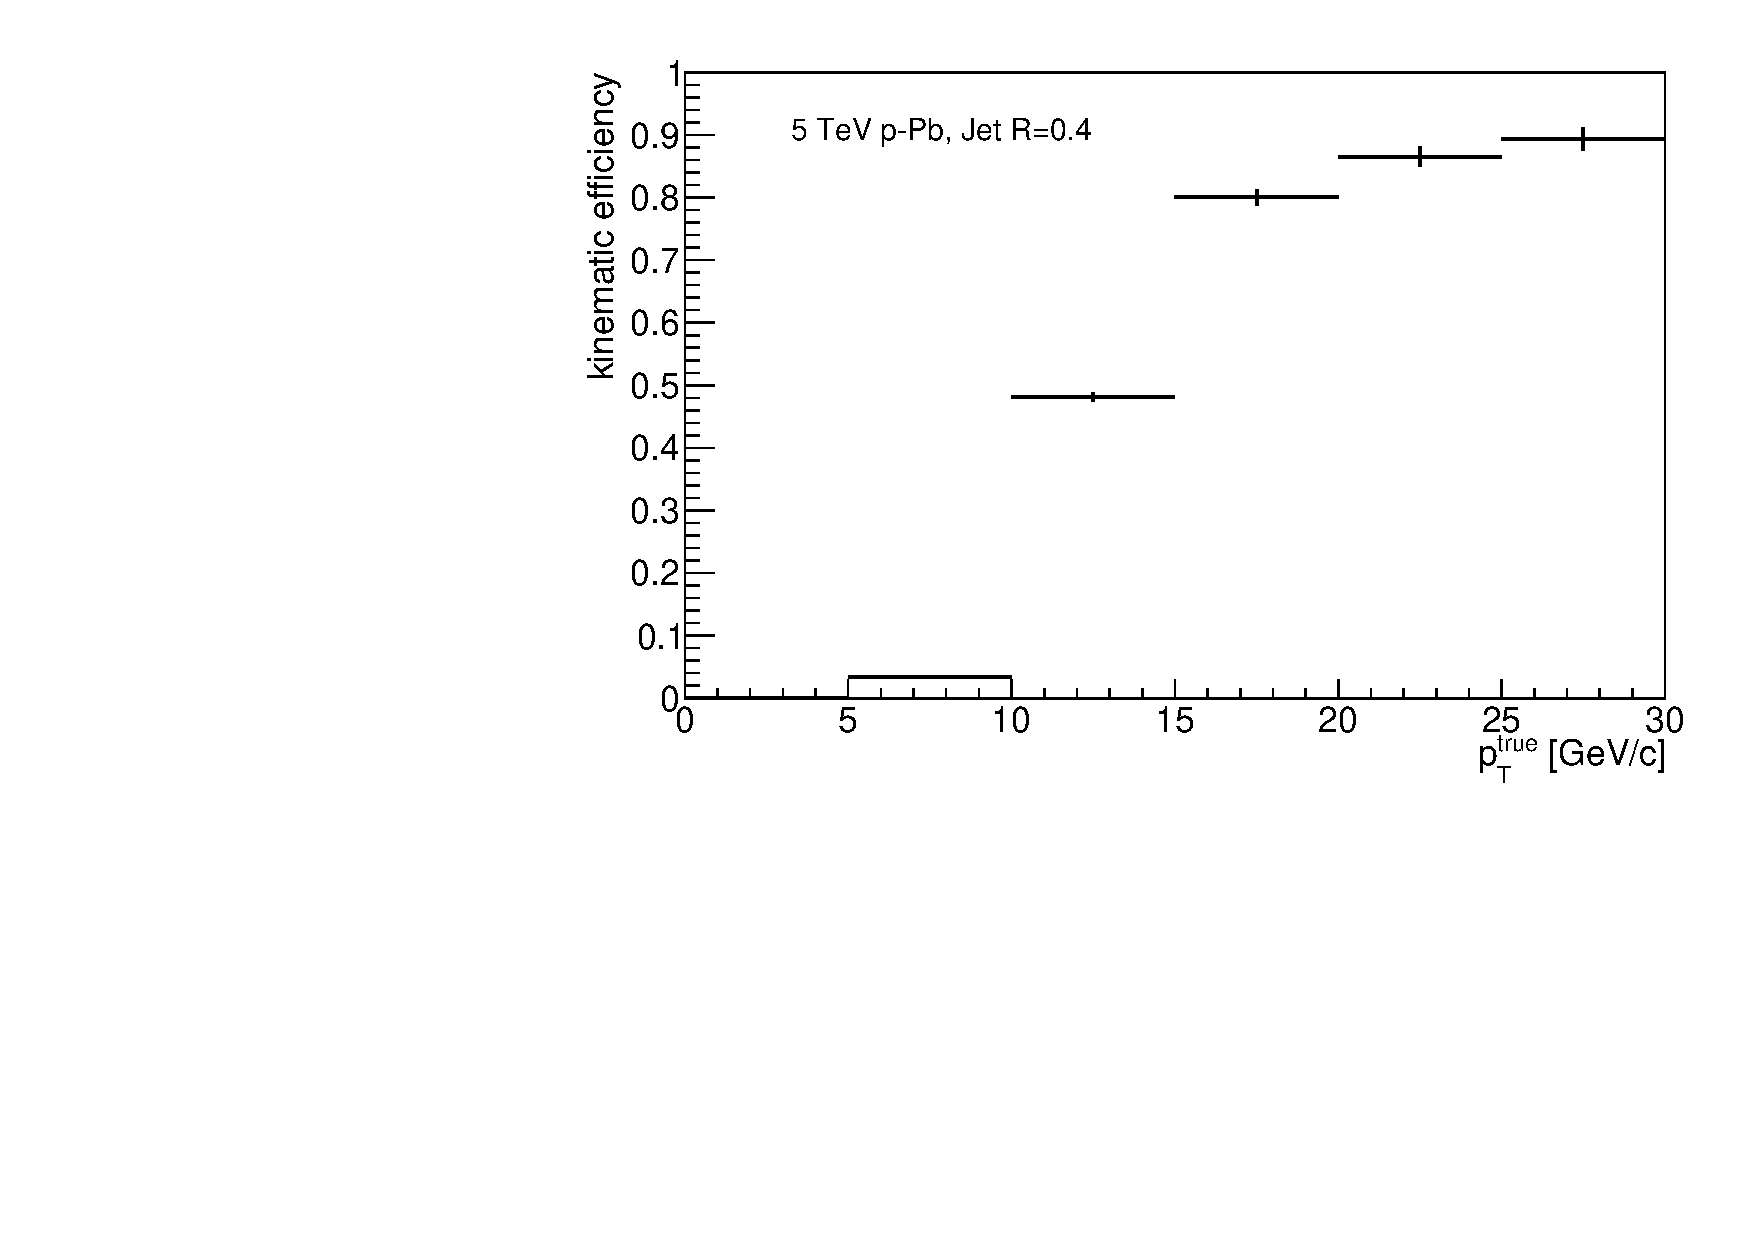
\includegraphics[width=0.49\textwidth]{JetResponse/KinematicEfficiencypPb}
\label{fig:kinematic_efficiency}
\caption{Kinematic efficiency for reconstructing generator-level jets with $\ptreco>$10 \GeVc, as a function of $\pttruth$. The jets have $|\eta^{\mathrm{reco}}|<0.5$. The error bar represents statistical uncertainty only. }
\end{figure}

Figure~\ref{fig:UnfoldedResultFinal} shows the result of the unfolding procedure, obtained using 4 iterations in the Bayesian method. The unfolded distribution agrees well with the prior distribution from \textsc{Pythia} photon+jet simulations. 

\begin{figure}
\center
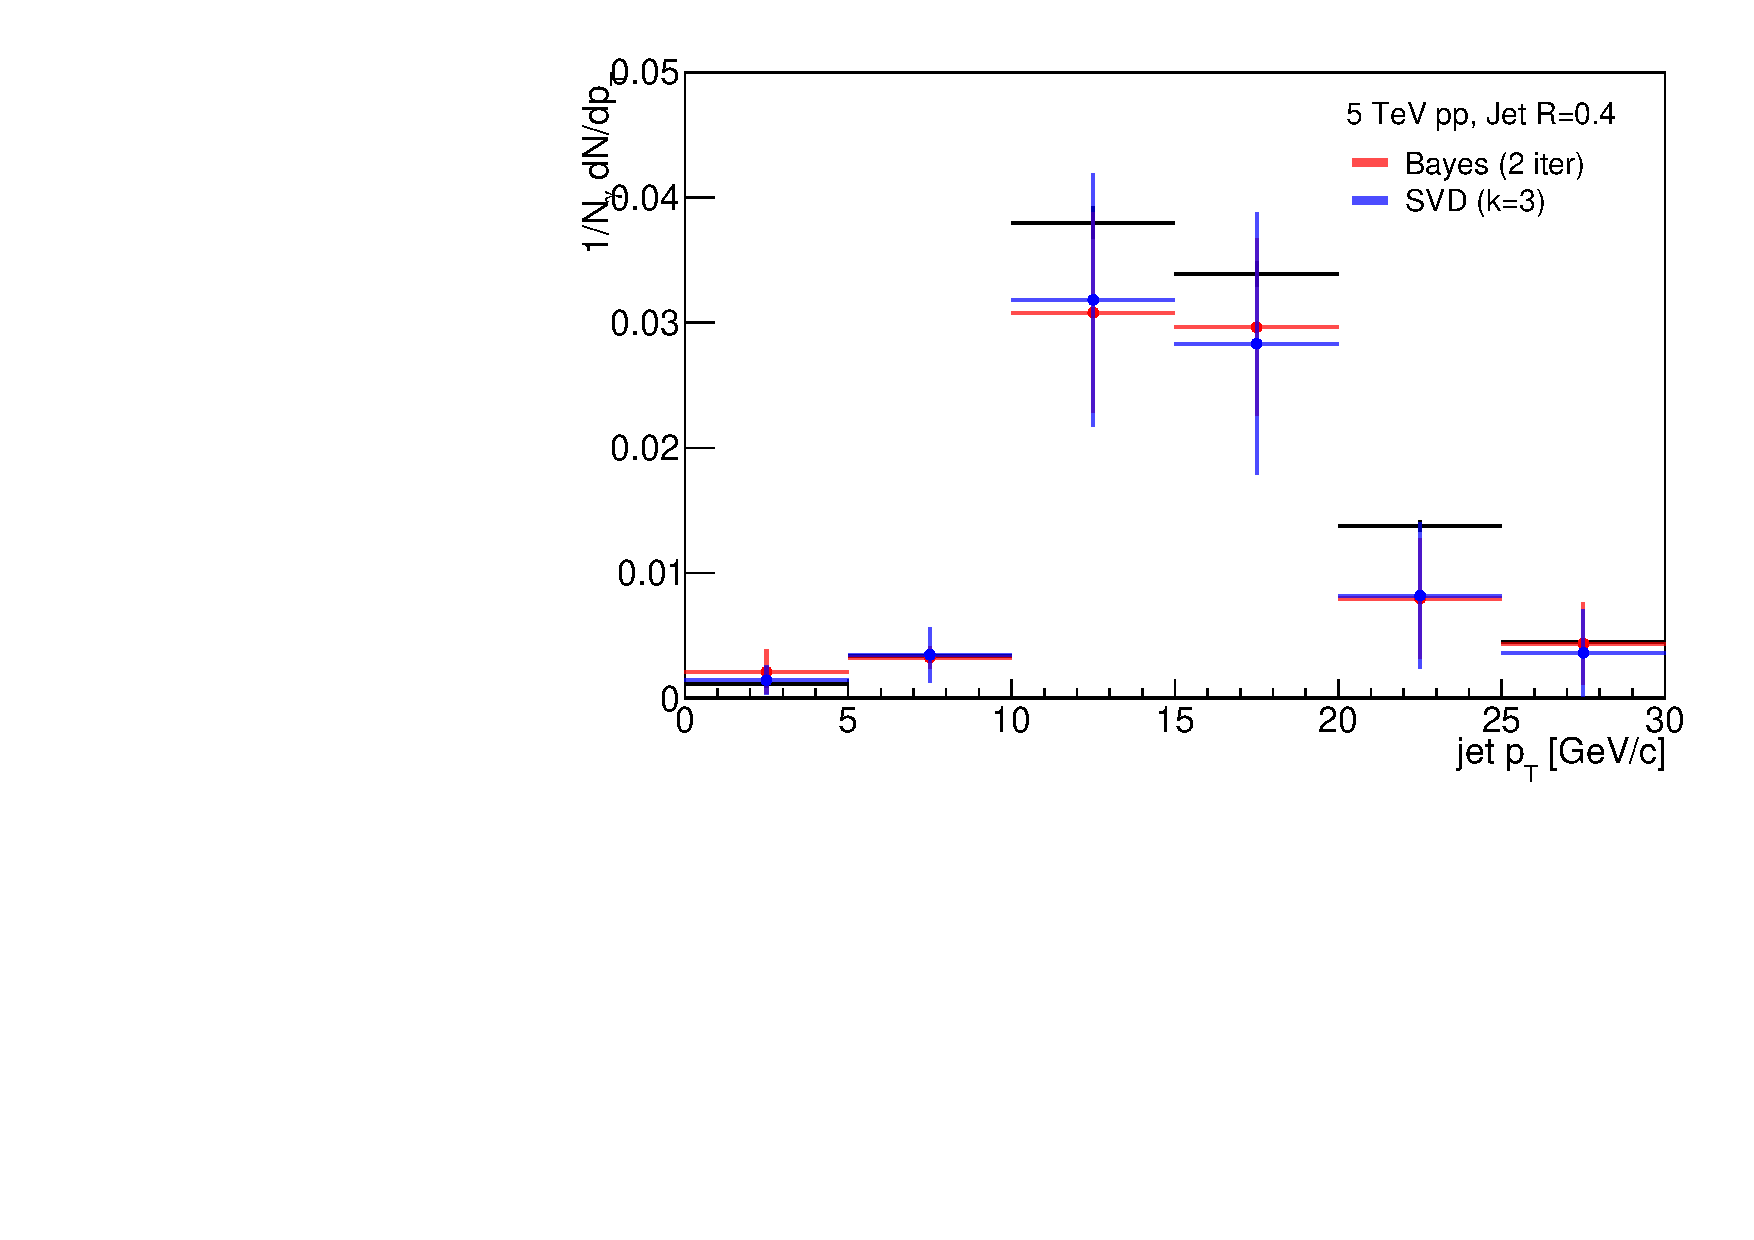
\includegraphics[width=0.49\textwidth]{JetResponse/Unfoldedresultpp}
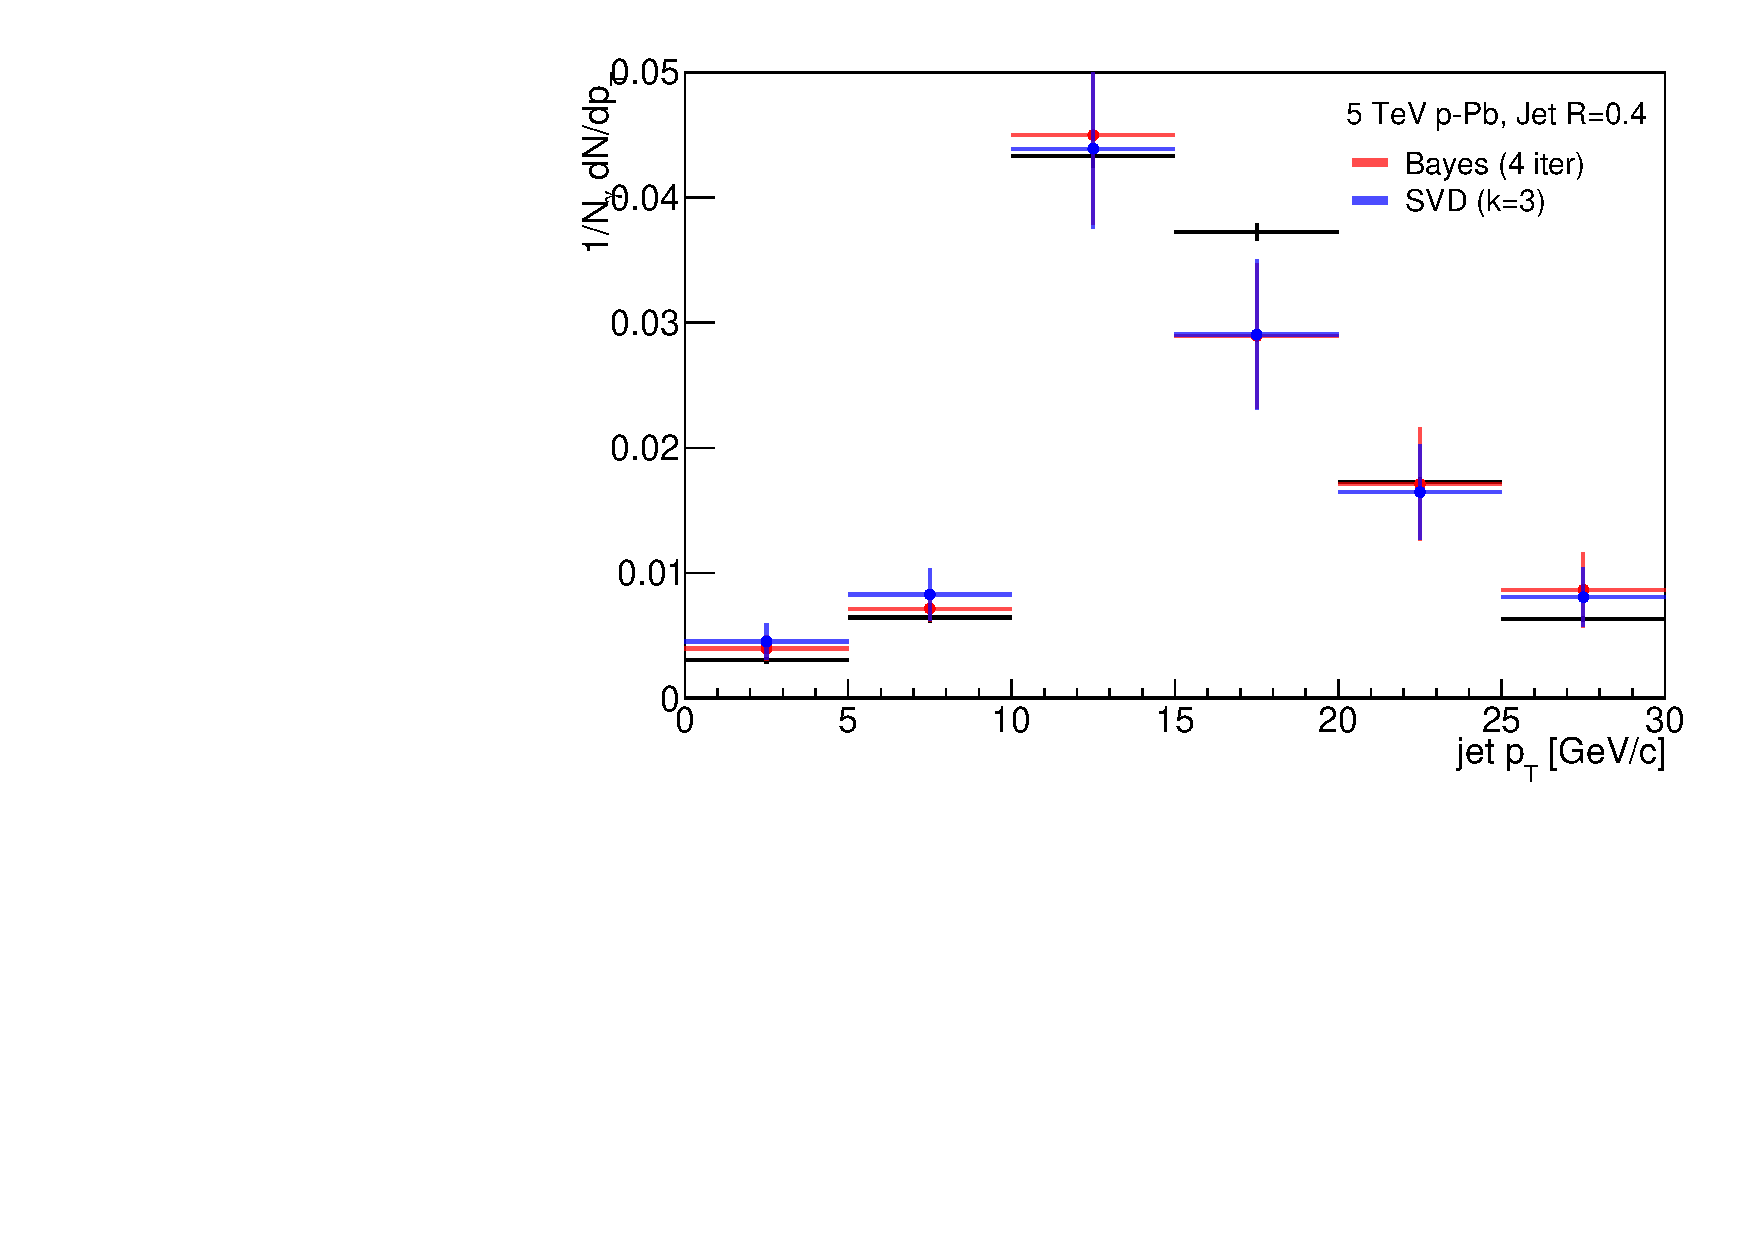
\includegraphics[width=0.49\textwidth]{JetResponse/UnfoldedresultpPb}
\caption{Unfolded jet $\pt$ distribution (in red) and prior used in the Bayesian unfolding (in black) and SVD (in blue). The error bar represents statistical uncertainty only.\label{fig:UnfoldedResultFinal}
}
\end{figure}

\begin{figure}
\center
	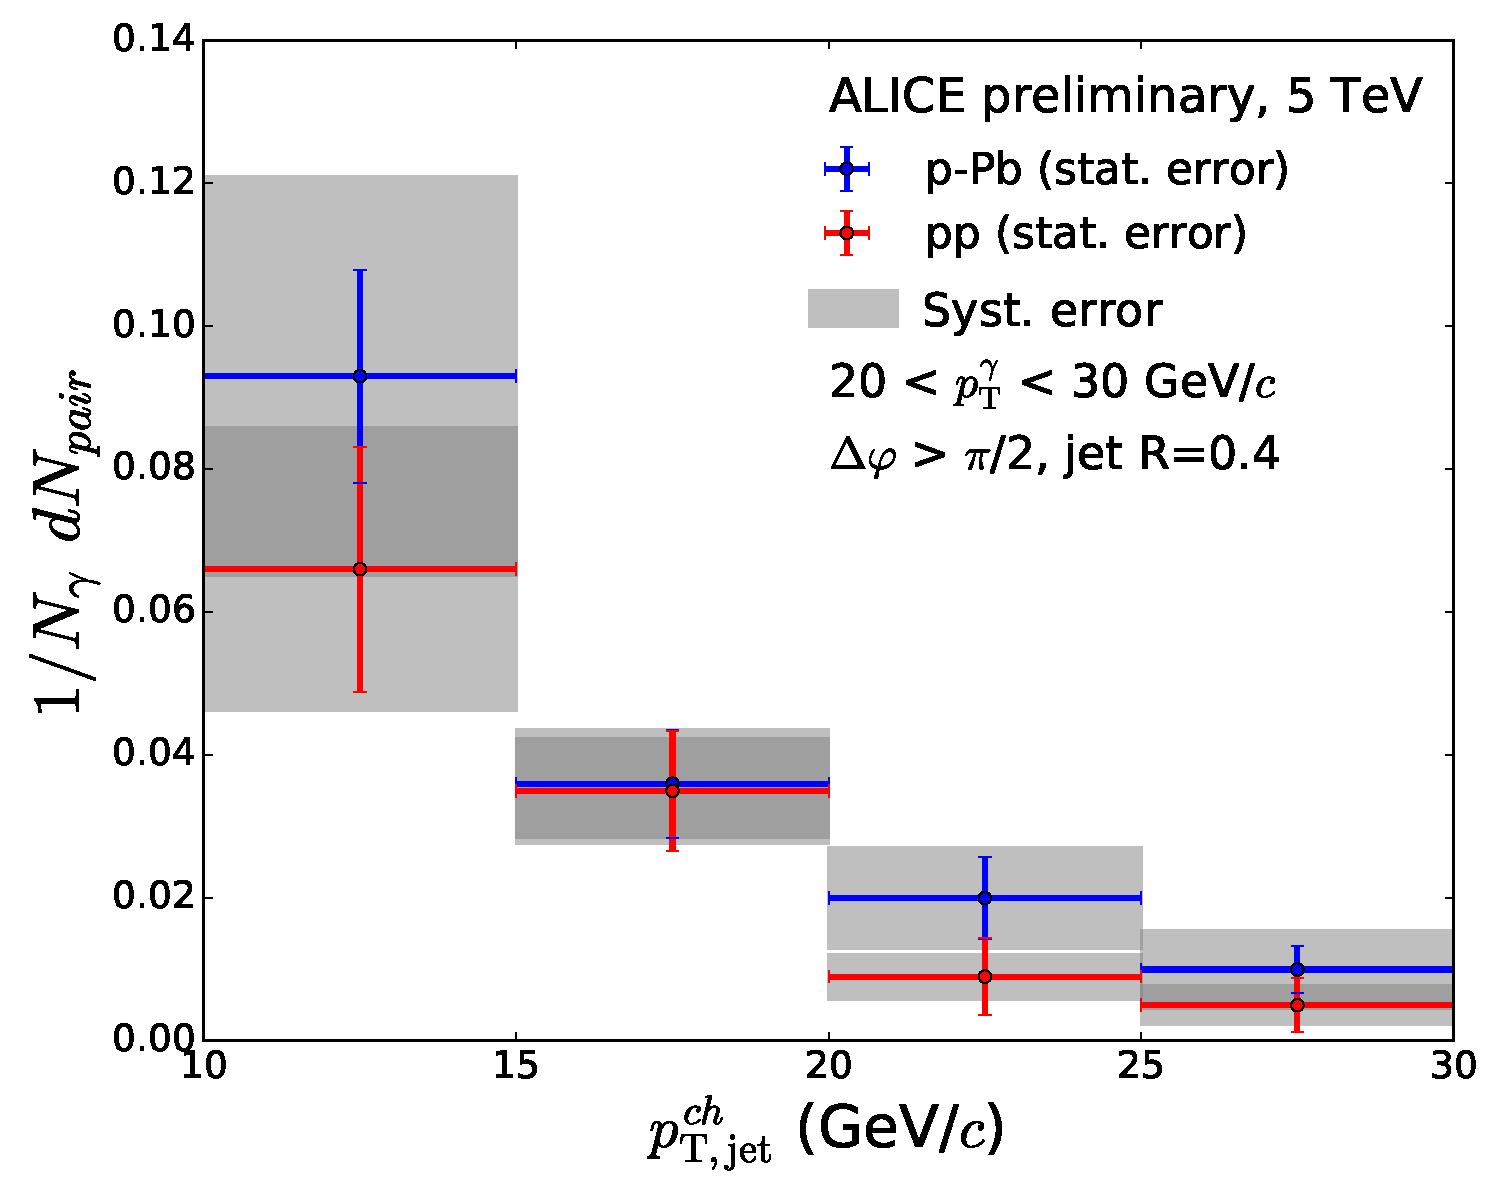
\includegraphics[width=0.6\textwidth]{JetResponse/Central_values.pdf}
	\caption{Fully corrected yield of jets per isolated photon as a function of jet transverse momentum. The error bars represent statistical uncertainties and the grey represent the systematic uncertainties. Due to the nature of the unfolding procedure, the systematic uncertainties are partially correlated bin to bin. Also, the statistical uncertainties are partially correlated bin to bin.}
	\label{fig:centralvalues}
\end{figure}

Figure~\ref{fig:PearsonMatrix} shows the normalized covariance matrix (i.e Pearson correlation coefficients) obtained form the unfolding procedure. The covariance matrix is mostly diagonal, at least for region above 10 \GeVc. The strong correlations present in the lower-left corner of the covariance matrix arise simply because that is a region with large statistical uncertainties and not to constrained by the measured data ({$\pt^{\mathrm{reco}}>10$} \GeVc).
\begin{figure}
\center
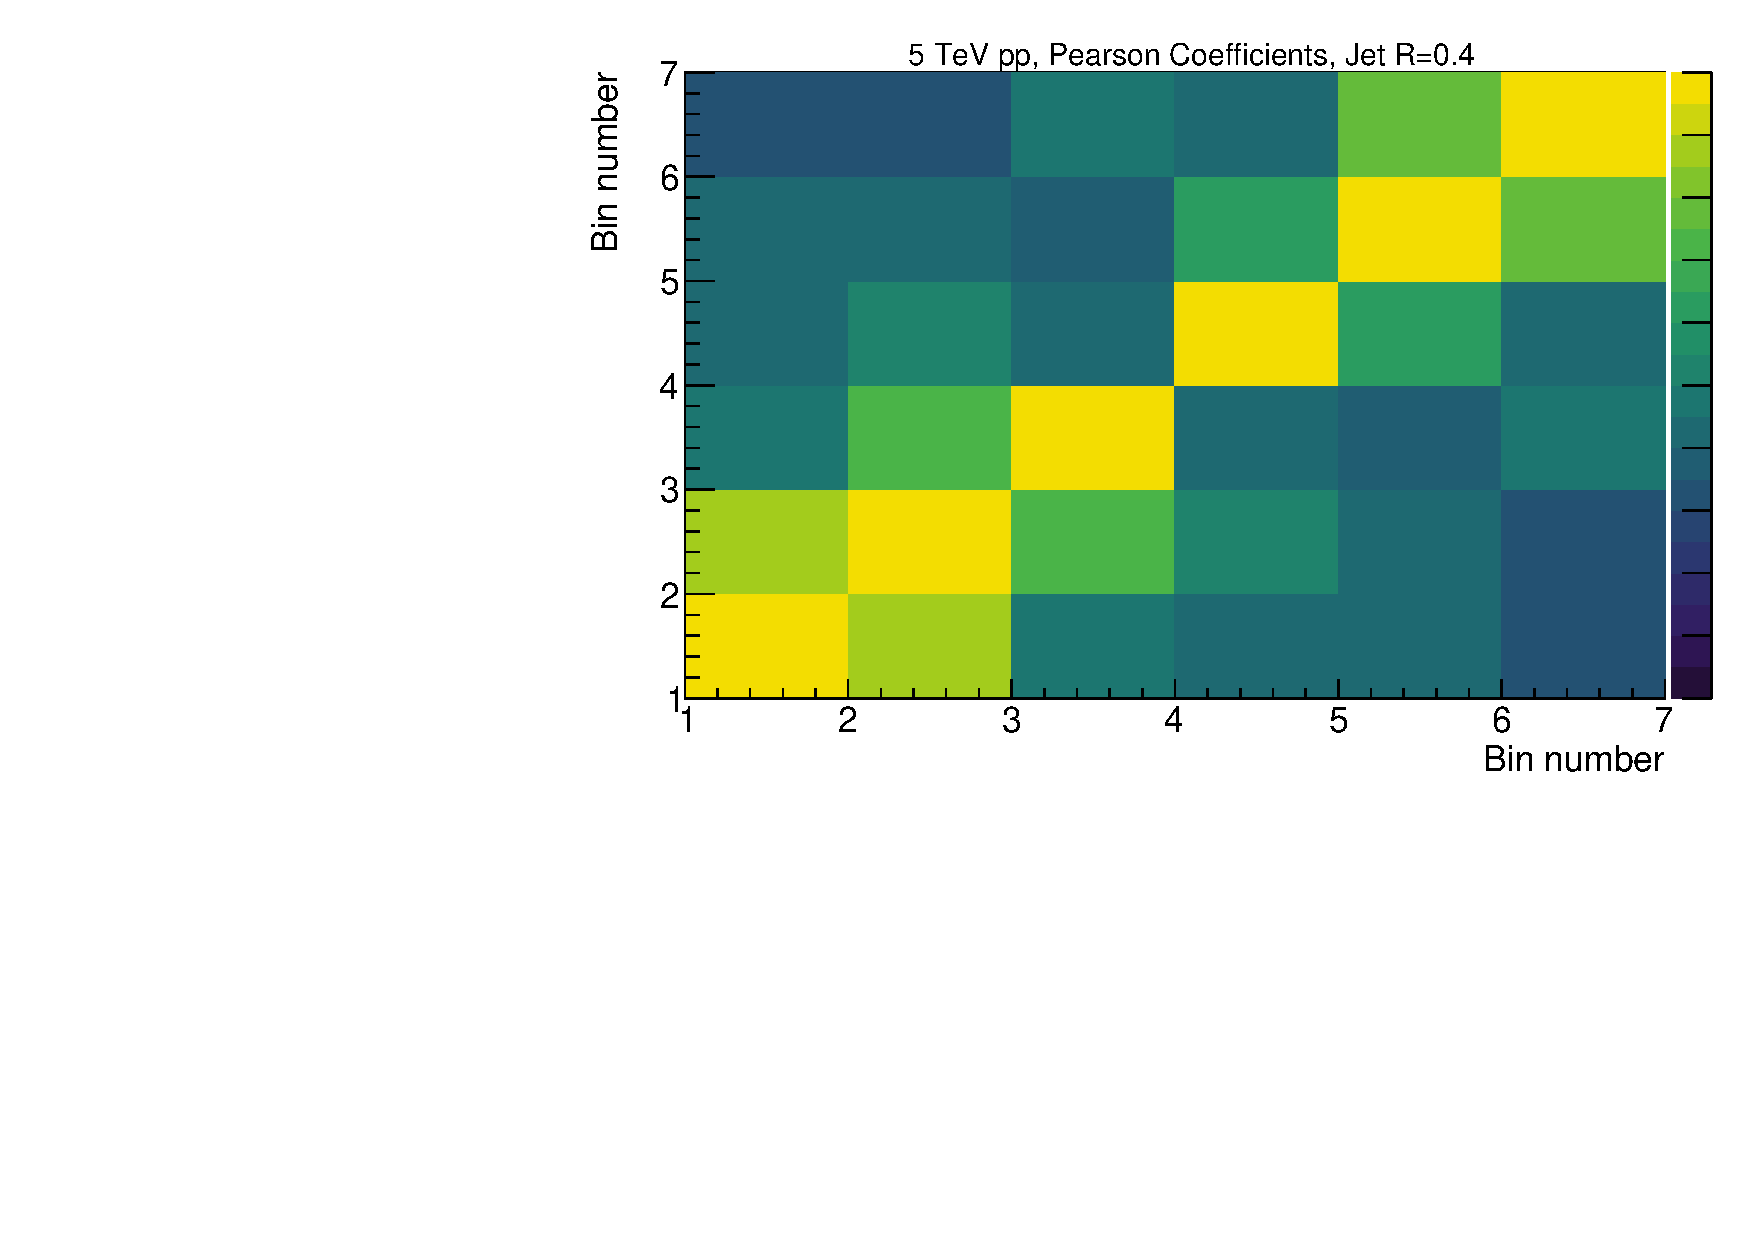
\includegraphics[width=0.49\textwidth]{JetResponse/Pearsonpp}
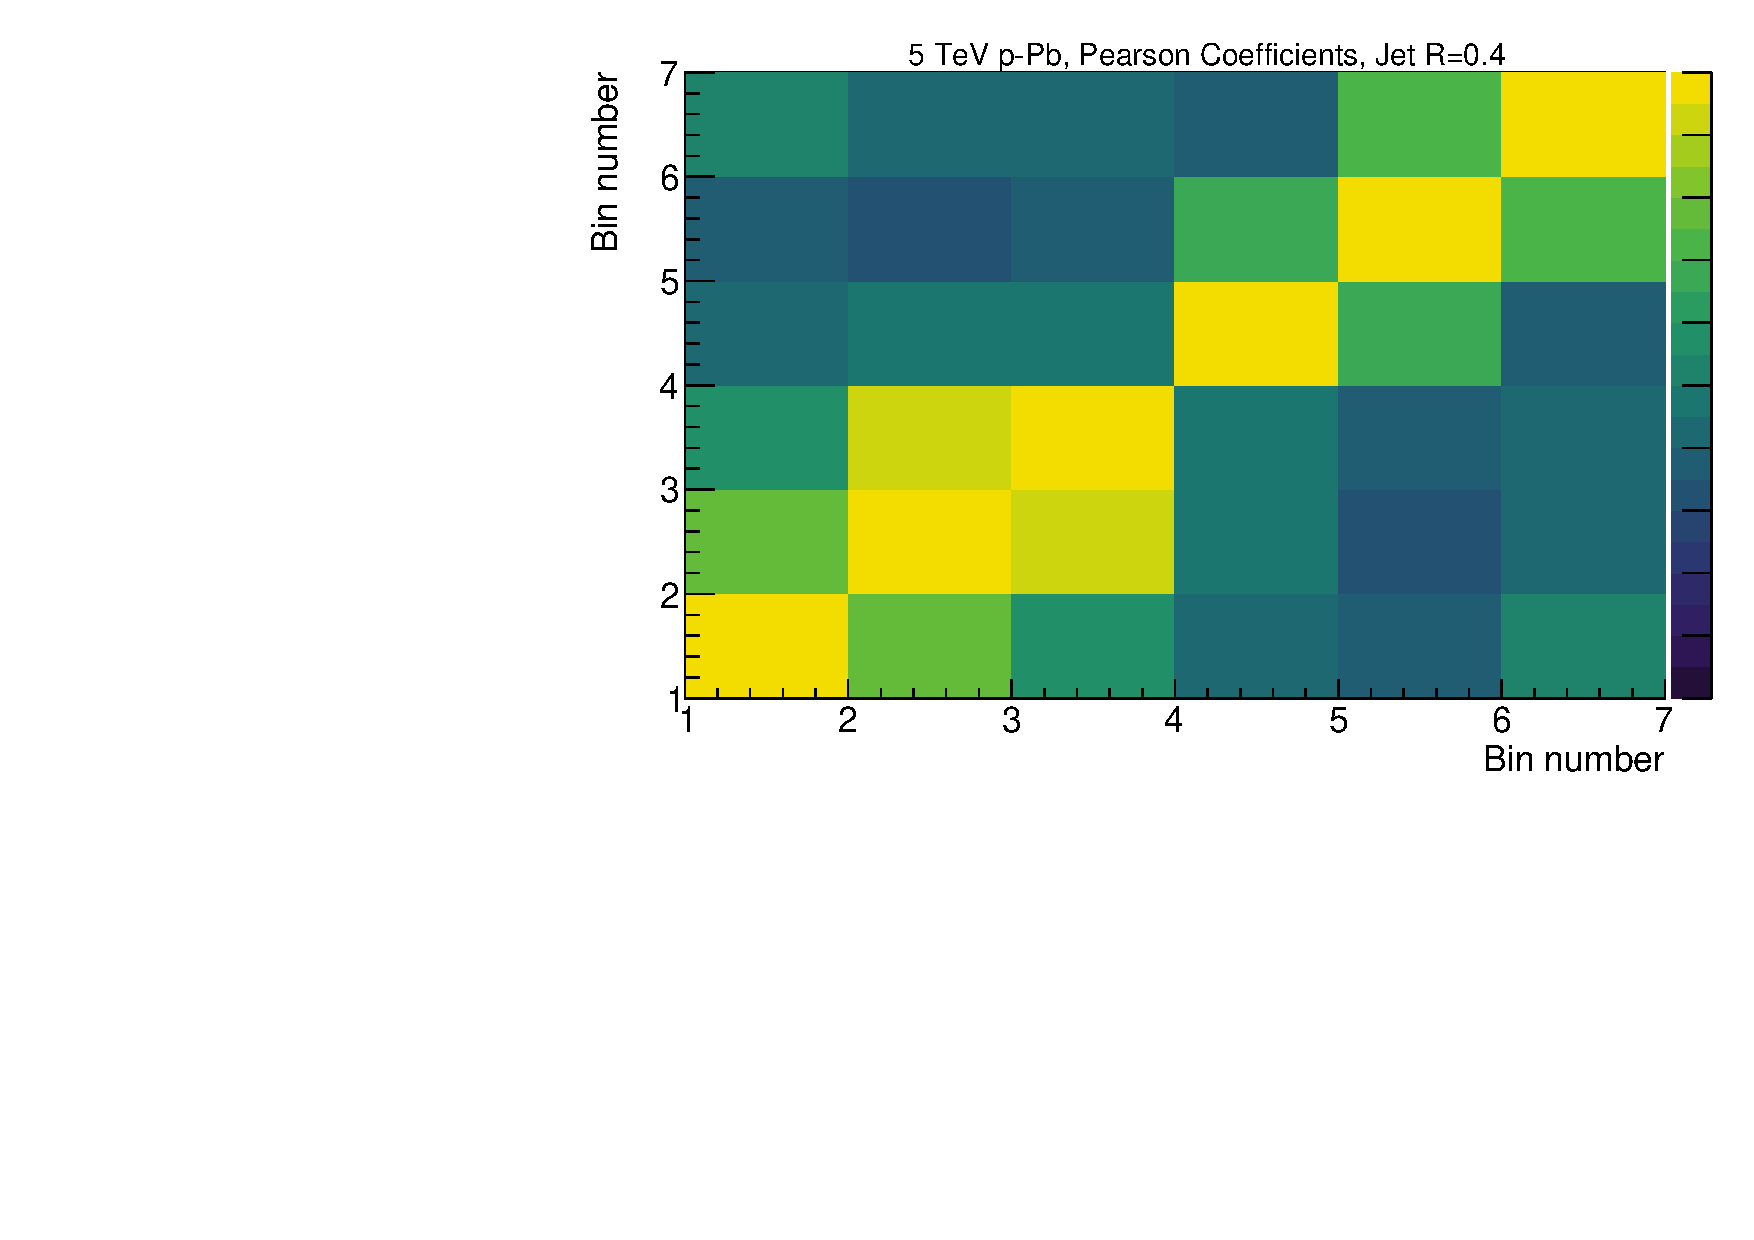
\includegraphics[width=0.49\textwidth]{JetResponse/PearsonpPb}
\label{fig:PearsonMatrix}
\caption{Pearson correlation coefficients, obtained from the covariance matrix that is the result of the unfolding procedure, for the jet $\pt$ spectrum. The axes represent bin numbers in the unfolded distribution. The maximum and minimum of the color scale are $+1.0$ and $-1.0$ respectively.}
\end{figure}

We check the result of our unfolding procedure by using alternative methods such as the ``Single-Value-Decomposition" method~\cite{Hocker:1995kb}, and the ``Iterative, Dynamically Stabilized" method~\cite{Malaescu:2011yg}, implemented in \textsc{RooUnfold} as the~\textsc{RooUnfoldSvd} and~\textsc{RooUnfoldIds} classes. All different methods yield consistent results. 

\subsubsection{Refolding check}
We perform a ``refolding'' check by taking the unfolded distribution and multiplying it with the response matrix shown in Figure~\ref{fig:JetPTUnfolding}, and comparing that to the reconstructed-level distribution. Figure~\ref{fig:Refolding} shows the comparison between reconstructed-level and refolded distributions for both pp and p-Pb data. No significant bias is observed. 

\begin{figure}
\center
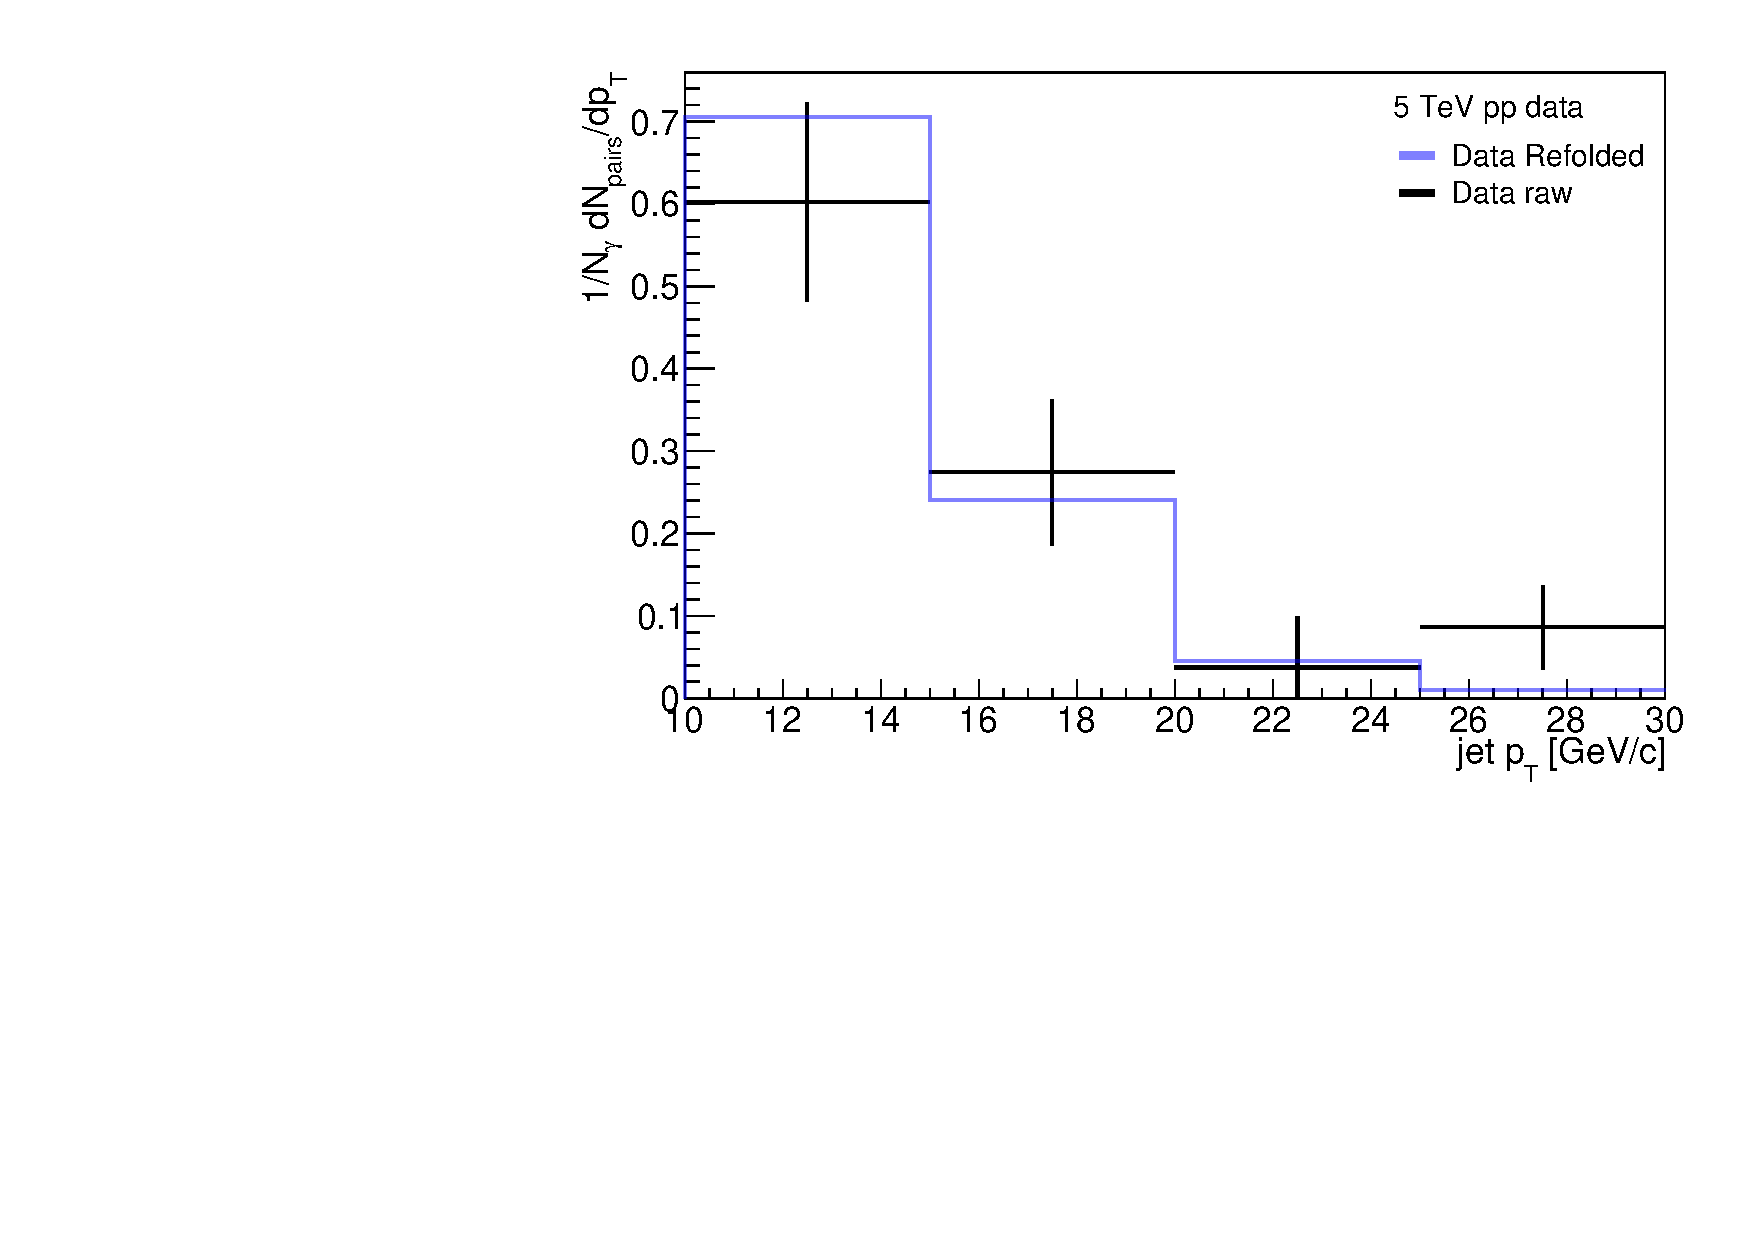
\includegraphics[width=0.49\textwidth]{JetResponse/RefoldingCheck_pp}
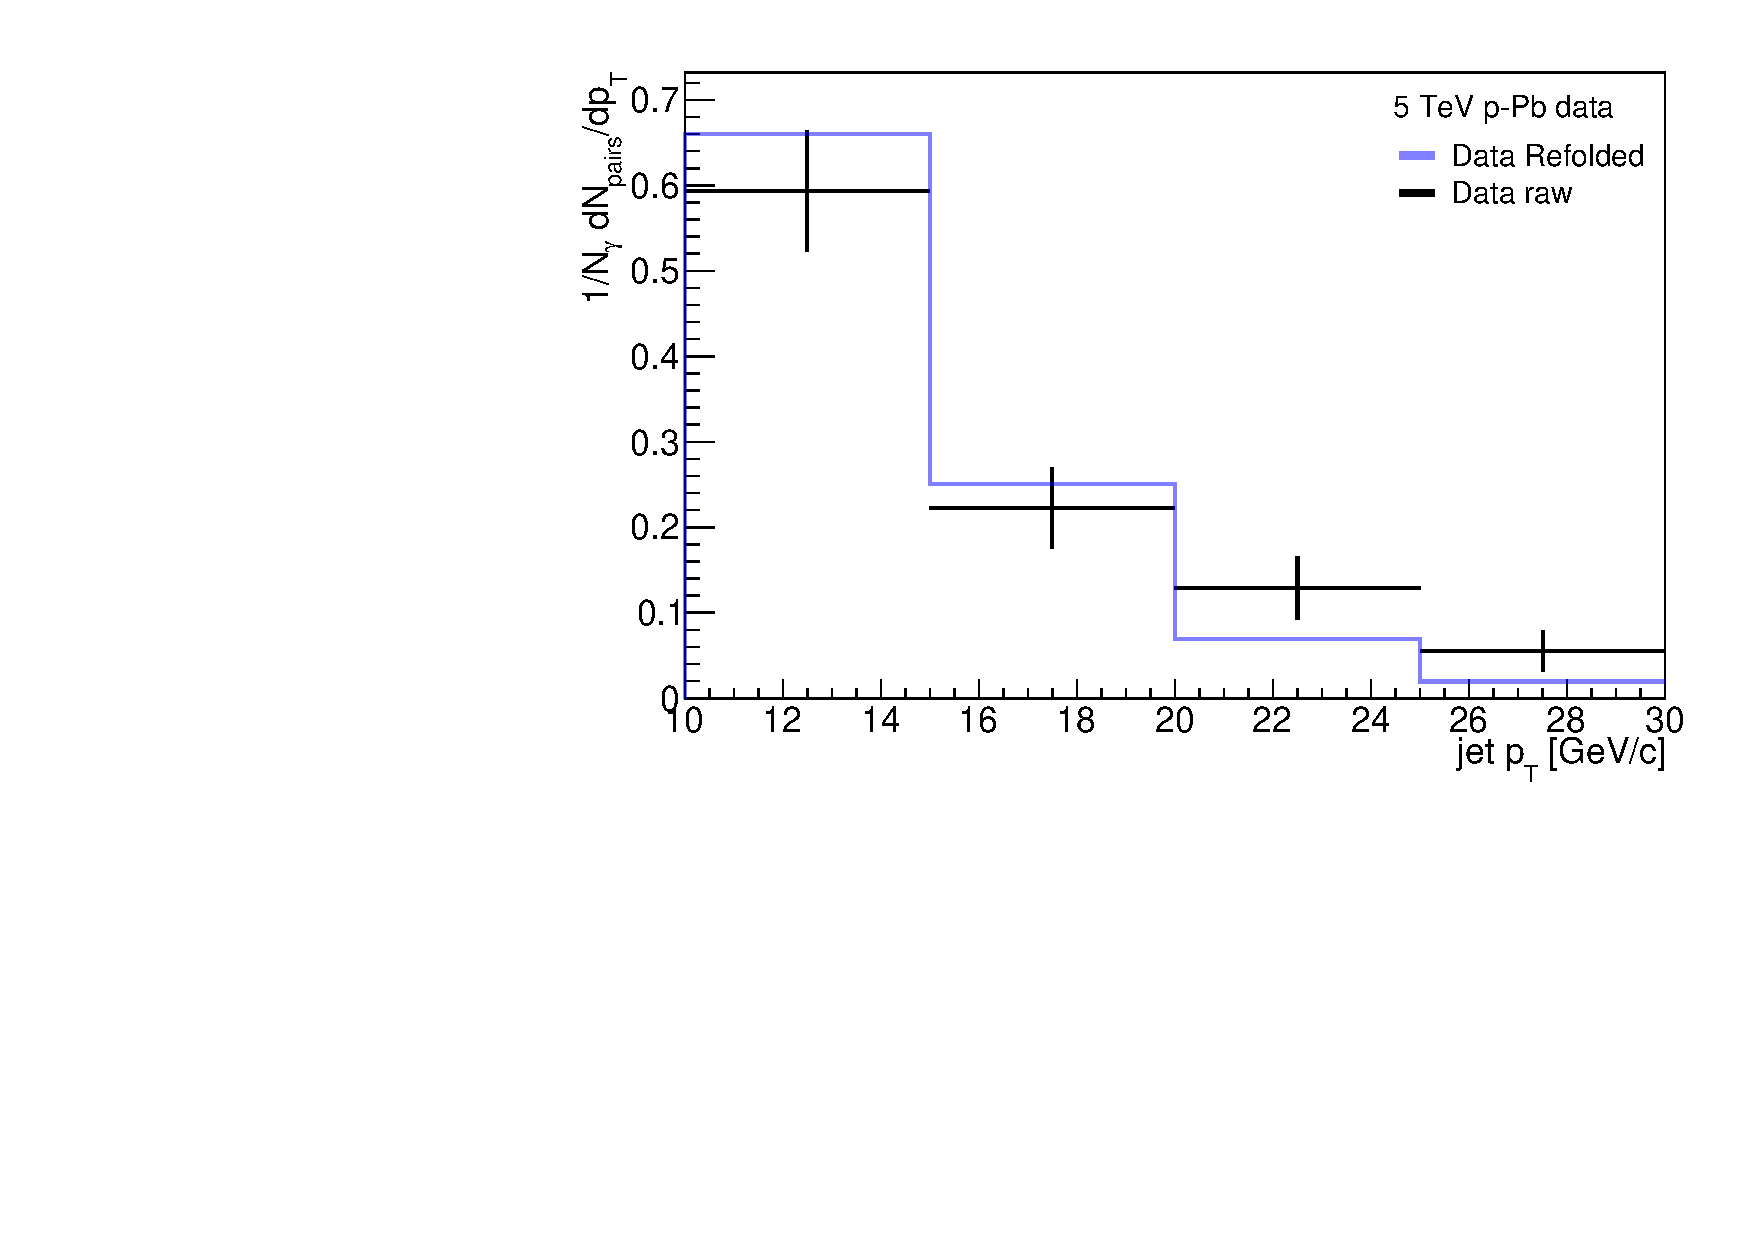
\includegraphics[width=0.49\textwidth]{JetResponse/RefoldingCheck_pPb}
\label{fig:Refolding}
\caption{Refolding check results}
\end{figure}

\FloatBarrier
\subsection{Photon Unfolding}
As stated in Section~\ref{sec:experimentalsetup}, the EMCAL energy resolution can be parametrized as $\sigma_{E}/E = 4.8\%/E\otimes 11.3\%/\sqrt{E}\otimes 1.7\%$ where the energy $E$ is given in units of GeV~\cite{Abeysekara:2010ze}. Thus for the photon $E_{\mathrm{T}}$ that we are relevant for this analysis, the relative energy resolution is at the level of a few percent. The response matrix for prompt photons obtained from \textsc{Pythia} photon+jet simulation, shown in Figure~\ref{fig:photonunfolding}, is strongly diagonal reflecting this fact.  
\begin{figure}
\centering
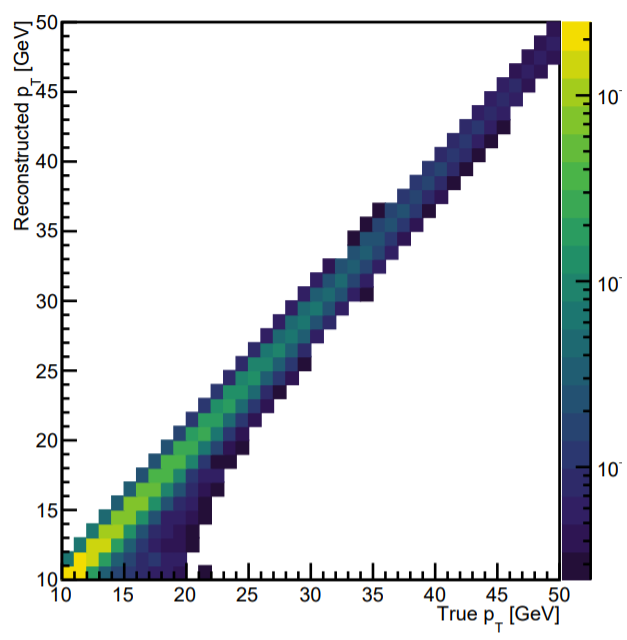
\includegraphics[width=0.40\textwidth]{JetResponse/PHOTONMATRIX}
\caption{Response matrix for prompt photons from photon+jet simulation. The response matrix is very close to being diagonal, so for illustration purposes we show the color code in logarithmic scale.}
\label{fig:photonunfolding}
\end{figure}

The smearing effects related to photon $\pt$ measurements are much smaller than the corresponding effects for jet $\pt$ measurements, so they have little relative impact in the measurements of $x_{J}$ and $x_{Obs}^{Pb}$ presented in this note. For simplicity (i.e, to avoid a two-dimensional unfolding procedure), we simply neglect the photon energy resolution. We cross-check this by varying the measured momentum of the photon $\pt$ by $\pm\sigma$. A similar approach was taken in previous hadron-jet measurements, where the hadron momentum resolution is also at the percent level.  